\documentclass{article}
\usepackage{arxiv}
\makeatletter
\@ifclassloaded{bioinfo}{%
    % work fine with Bioinformatics
    \usepackage{lmodern}
    \usepackage{color}
    \usepackage{float}
    \usepackage{url}            % simple URL typesetting
    \usepackage{nicefrac}       % compact symbols for 1/2, etc.
    \usepackage{microtype}      % micro-typography
    \usepackage{amsfonts}       % blackboard math symbols
    \usepackage{amsmath}
    \usepackage{mathtools}
    \usepackage{amssymb}
    \usepackage{amsthm}
    \usepackage{bbm}
    \usepackage{bm}
    \usepackage{longtable}
    \usepackage[ruled,vlined,linesnumbered]{algorithm2e}
    \usepackage{placeins}
}{%
    % work fine with Bioinformatics
    \usepackage{lmodern}
    \usepackage{color}
    \usepackage{float}
    \usepackage{url}            % simple URL typesetting
    \usepackage{nicefrac}       % compact symbols for 1/2, etc.
    \usepackage{microtype}      % micro-typography
    \usepackage{amsfonts}       % blackboard math symbols
    \usepackage{amsmath}
    \usepackage{mathtools}
    \usepackage{amssymb}
    \usepackage{amsthm}
    \usepackage{bbm}
    \usepackage{bm}
    \usepackage{longtable}
    \usepackage[ruled,vlined,linesnumbered]{algorithm2e}
    \usepackage{placeins}
    \usepackage{multibib}
    \newcites{SM}{Supplementary Information References}

    % cause issues with Bioinformatics
    \usepackage[utf8]{inputenc} % allow utf-8 input
    \usepackage[T1]{fontenc}    % use 8-bit T1 fonts
    \usepackage{xcolor}
    \usepackage{xr-hyper}
    \usepackage{hyperref}       % hyperlinks
    \usepackage{booktabs}       % professional-quality tables
    \usepackage{graphicx}
    \usepackage[square,numbers]{natbib}
    \usepackage{array}          % for text wrap in appendix tables
    \newcolumntype{L}{>{\centering\arraybackslash}m{3cm}}
}
\makeatother

\makeatletter\renewcommand*{\fps@figure}{H}\makeatother
\DeclareMathOperator*{\argmax}{argmax}
\DeclareMathOperator*{\argmin}{argmin}
\newcommand{\beginsupplement}{%
        \setcounter{table}{0}
        \renewcommand{\thetable}{S\arabic{table}}%
        \setcounter{figure}{0}
        \renewcommand{\thefigure}{S\arabic{figure}}%
        \setcounter{section}{0}
        \renewcommand{\thesection}{S\arabic{section}}%
     }
\externaldocument{main}
\begin{document}
\beginsupplement
\section*{Supplementary Information}

\section{Algorithm for Cross-Validated scPCA}

\begin{algorithm}[!htbp]\label{algo2}
  \dontprintsemicolon
  %\setalgolined
  \linesnotnumbered
  \KwResult{Produces a sparse low-dimensional representation of the target data,
    $\mathbf{X}_{n \times p}$, by contrasting the variation of
    $\mathbf{X}_{n \times p}$ and some background data, $\mathbf{Y}_{m \times p}$,
    while applying an $\ell_1$ penalty to the loadings generated by cPCA.}
  \SetKwInOut{Input}{Input}\SetKwInOut{Output}{Output}
  \Input{
  \begin{itemize}
    \item[] target dataset: $\mathbf{X}$
    \item[] background dataset: $\mathbf{Y}$
    \item[] binary variable indicating whether to column-scale the data:
      \texttt{scale}
    \item[] vector of possible contrastive parameters:
      $\gamma = (\gamma_1, \ldots, \gamma_s)$
    \item[] vector of possible $\ell_1$ penalty parameters: $\lambda_1 = (\lambda_{1,1}, \ldots, \lambda_{1, d})$
    \item[] number of sparse contrastive principal components to compute: $k$
    \item[] clustering method: \texttt{cluster\_meth}
    \item[] number of clusters: \texttt{ncluster}
    \item[] number of cross-validation folds: $V$
  \end{itemize}
  }
  \BlankLine
  For $\mathbf{X}_{n \times p}$, randomly partition the index set $\{1, \ldots,
  n\}$ into $V$ validation sets, $\mathcal{V}_1^x, \ldots, \mathcal{V}_V^x$, of (approximately) the
  same size (i.e., $\bigcup_{v=1}^V \mathcal{V}_v^x = \{1, \ldots, n\}$;
  $\mathcal{V}_v^x
  \cap \mathcal{V}_{v'}^x = \emptyset, \quad \forall v,v' \in \{1, \ldots, V\}$).
  Denote the corresponding training sets by $\mathcal{T}_v^x = \{1, \ldots, n\}
  \setminus \mathcal{V}_v^x$. For $\mathbf{Y}_{m \times p}$, randomly partition the
  index set $\{1, \ldots, m\}$ into $V$ validation sets, $\mathcal{V}_1^y, \ldots,
  \mathcal{V}_V^y$, of (approximately) the same size (i.e., $\bigcup_{v=1}^V \mathcal{V}_v^y = \{1,
      \ldots, m\}$; $\mathcal{V}_v^y \cap \mathcal{V}_{v'}^y = \emptyset, \quad
      \forall
      v,v' \in \{1, \ldots, V\}$). Denote the corresponding training sets by
  $\mathcal{T}_v^y = \{1, \ldots, m\} \setminus \mathcal{V}_v^y$. Denote by
$\mathbf{X}_{\mathcal{T}_v^x}$ the $\left(n - \lvert \mathcal{T}_v^x \rvert\right)
  \times p$ submatrix of $\mathbf{X}$ for training set $\mathcal{T}_v^x$ and by
$\mathbf{Y}_{\mathcal{T}_v^y}$ the $\left(m - \lvert \mathcal{T}_v^y \rvert\right)
  \times p$ submatrix of $\mathbf{Y}$ for training set $\mathcal{T}^y_v$. Define similarly
  $\mathbf{X}_{\mathcal{V}_v^x}$ and $\mathbf{Y}_{\mathcal{V}_v^y}$ for the validation
  sets. Note that $\mathbf{Y}_{\mathcal{V}_v^y}$ is defined explicitly solely to
  avoid ambiguity; it plays no role in subsequent developments.\; \BlankLine
  \For{each $v$ in $\{1, \ldots, V\}$}{
    Center (and \texttt{scale} if so desired) the columns of
      $\{\mathbf{X}_{\mathcal{T}_v^x}, \mathbf{Y}_{\mathcal{T}_v^y} \}$ and
      $\{\mathbf{X}_{\mathcal{V}_v^x}, \mathbf{Y}_{\mathcal{V}_v^y} \}$\;
  Compute the empirical covariance matrices:
    $\mathbf{C_X}_{p \times p} \coloneqq \frac{1}{\lvert \mathcal{T}_v^x
    \rvert}\mathbf{X_{\mathcal{T}_v^x}}^\top\mathbf{X_{\mathcal{T}_v^x}}, \;
  \mathbf{C_Y}_{p \times p} \coloneqq \frac{1}{\lvert \mathcal{T}_v^y
    \rvert}\mathbf{Y_{\mathcal{T}_v^y}}^\top\mathbf{Y_{\mathcal{T}_v^y}}$\;
  \For{each $\gamma_i \in \gamma$}{
    \For{each $\lambda_{1,j} \in \lambda_1$}{
      Compute the contrastive covariance matrix $\mathbf{C}_{\gamma_i}=\mathbf{C_X} -
      \gamma_i \mathbf{C_Y}$\;
      Compute the positive-semidefinite approximation of $\mathbf{C}_{\gamma_i}$, $\widetilde{\mathbf{C}}_{\gamma_i}$\;
      Apply SPCA to $\widetilde{\mathbf{C}}_{\gamma_i}$ for $k$ components with $\ell_1$ penalty $\lambda_{1, j}$\;
      Generate a low-dimensional representation of the target validation set by
        projecting $\mathbf{X}_{\mathcal{V}_v^x}$ on the sparse loadings of SPCA\;
      Normalize the low-dimensional representation produced to be on the unit hypercube\;
      Cluster the normalized low-dimensional representation using \texttt{cluster\_meth} with \texttt{ncluster}\;
      Compute and record the clustering strength criterion associated with $(\gamma_i, \lambda_{1, j})$ \;
    }
  }
  }
  Identify the combination of hyperparameters maximizing the cross-validated
  mean (across all folds $\{1, \ldots, V\}$) of the clustering strength
  criterion: $\gamma^{\star},\: \lambda_1^{\star}$ \;
  \Output{The low-dimensional representation of the target data given by
    $(\gamma^{\star}, \lambda_1^{\star})$, a $n \times k$ matrix;
    the $p \times k$ matrix of loadings given by $(\gamma^{\star},
    \lambda_1^{\star})$; contrastive parameter $\gamma^{\star}$;
    $\ell_1$ penalty parameter $\lambda_1^{\star}$
  }
  \caption{Cross-validated scPCA}
\end{algorithm}

\FloatBarrier

\newpage

\section{Contrastive Parameter Intuition}

\begin{figure}[!htbp]
    \centering
    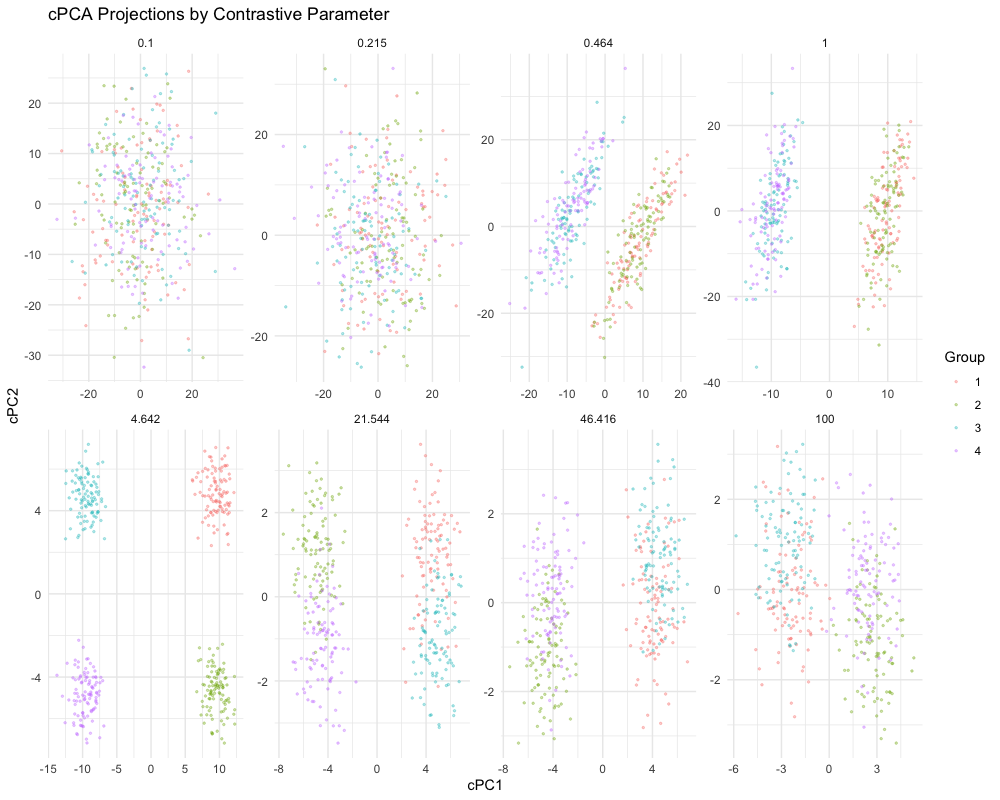
\includegraphics[width=0.9\textwidth]{figures/cpca_example_plot}
    \caption{
    {\em Effect of contrastive parameter for cPCA.}
    cPCA as implemented by Abid et al. was applied to a simulated dataset of $n=400$ observations, split across 4 groups, with $p=30$ variables. The first 10 variables are distributed as $N(0, 10)$ for all observations. Variables 11
    through 20 are distributed as $N(0, 1)$ for Groups 1 an 2, and as $N(3, 1)$
    for Groups 3 and 4. Variables 21 through 30 are distributed as $N(-3, 1)$
    for Groups 1 and 3, and as $N(0, 1)$ for Groups 2 and 4. cPCA also takes
    as input a background dataset of $m=400$ observations, with $p=30$
    variables, where the first 10 variables are distributed as $N(0, 10)$, the
    following 10 as $N(0, 3)$, and the remaining 10 as $N(0, 1)$. The results
    of cPCA are then presented for eight increasing values of the contrastive
    parameter $\gamma$, selected using the technique described by Abid et al. For the smaller values of the contrastive parameter, the
    noise contained in the first 10 variables of the target data dominates the
    signal contained in variables 11 through 30. As the contrastive parameter
    increases, the signal in the target data set is unmasked. However, once the
    contrastive parameter value becomes larger than $\approx 20$, the
    distinction between groups becomes increasingly poor; the variation
    contained in the background data begins to dominate the variation contained
    in the target data. A virtually identical dataset is presented in the
    supplementary material of Abid et al. }
    \label{contrastive_par}
\end{figure}

\FloatBarrier

\newpage

\section{Simulated Data}

See Section 3.1 %\ref{sim_scRNA-seq}
for information on the simulation model and dataset.

\begin{figure}[!htbp]
    \centering
    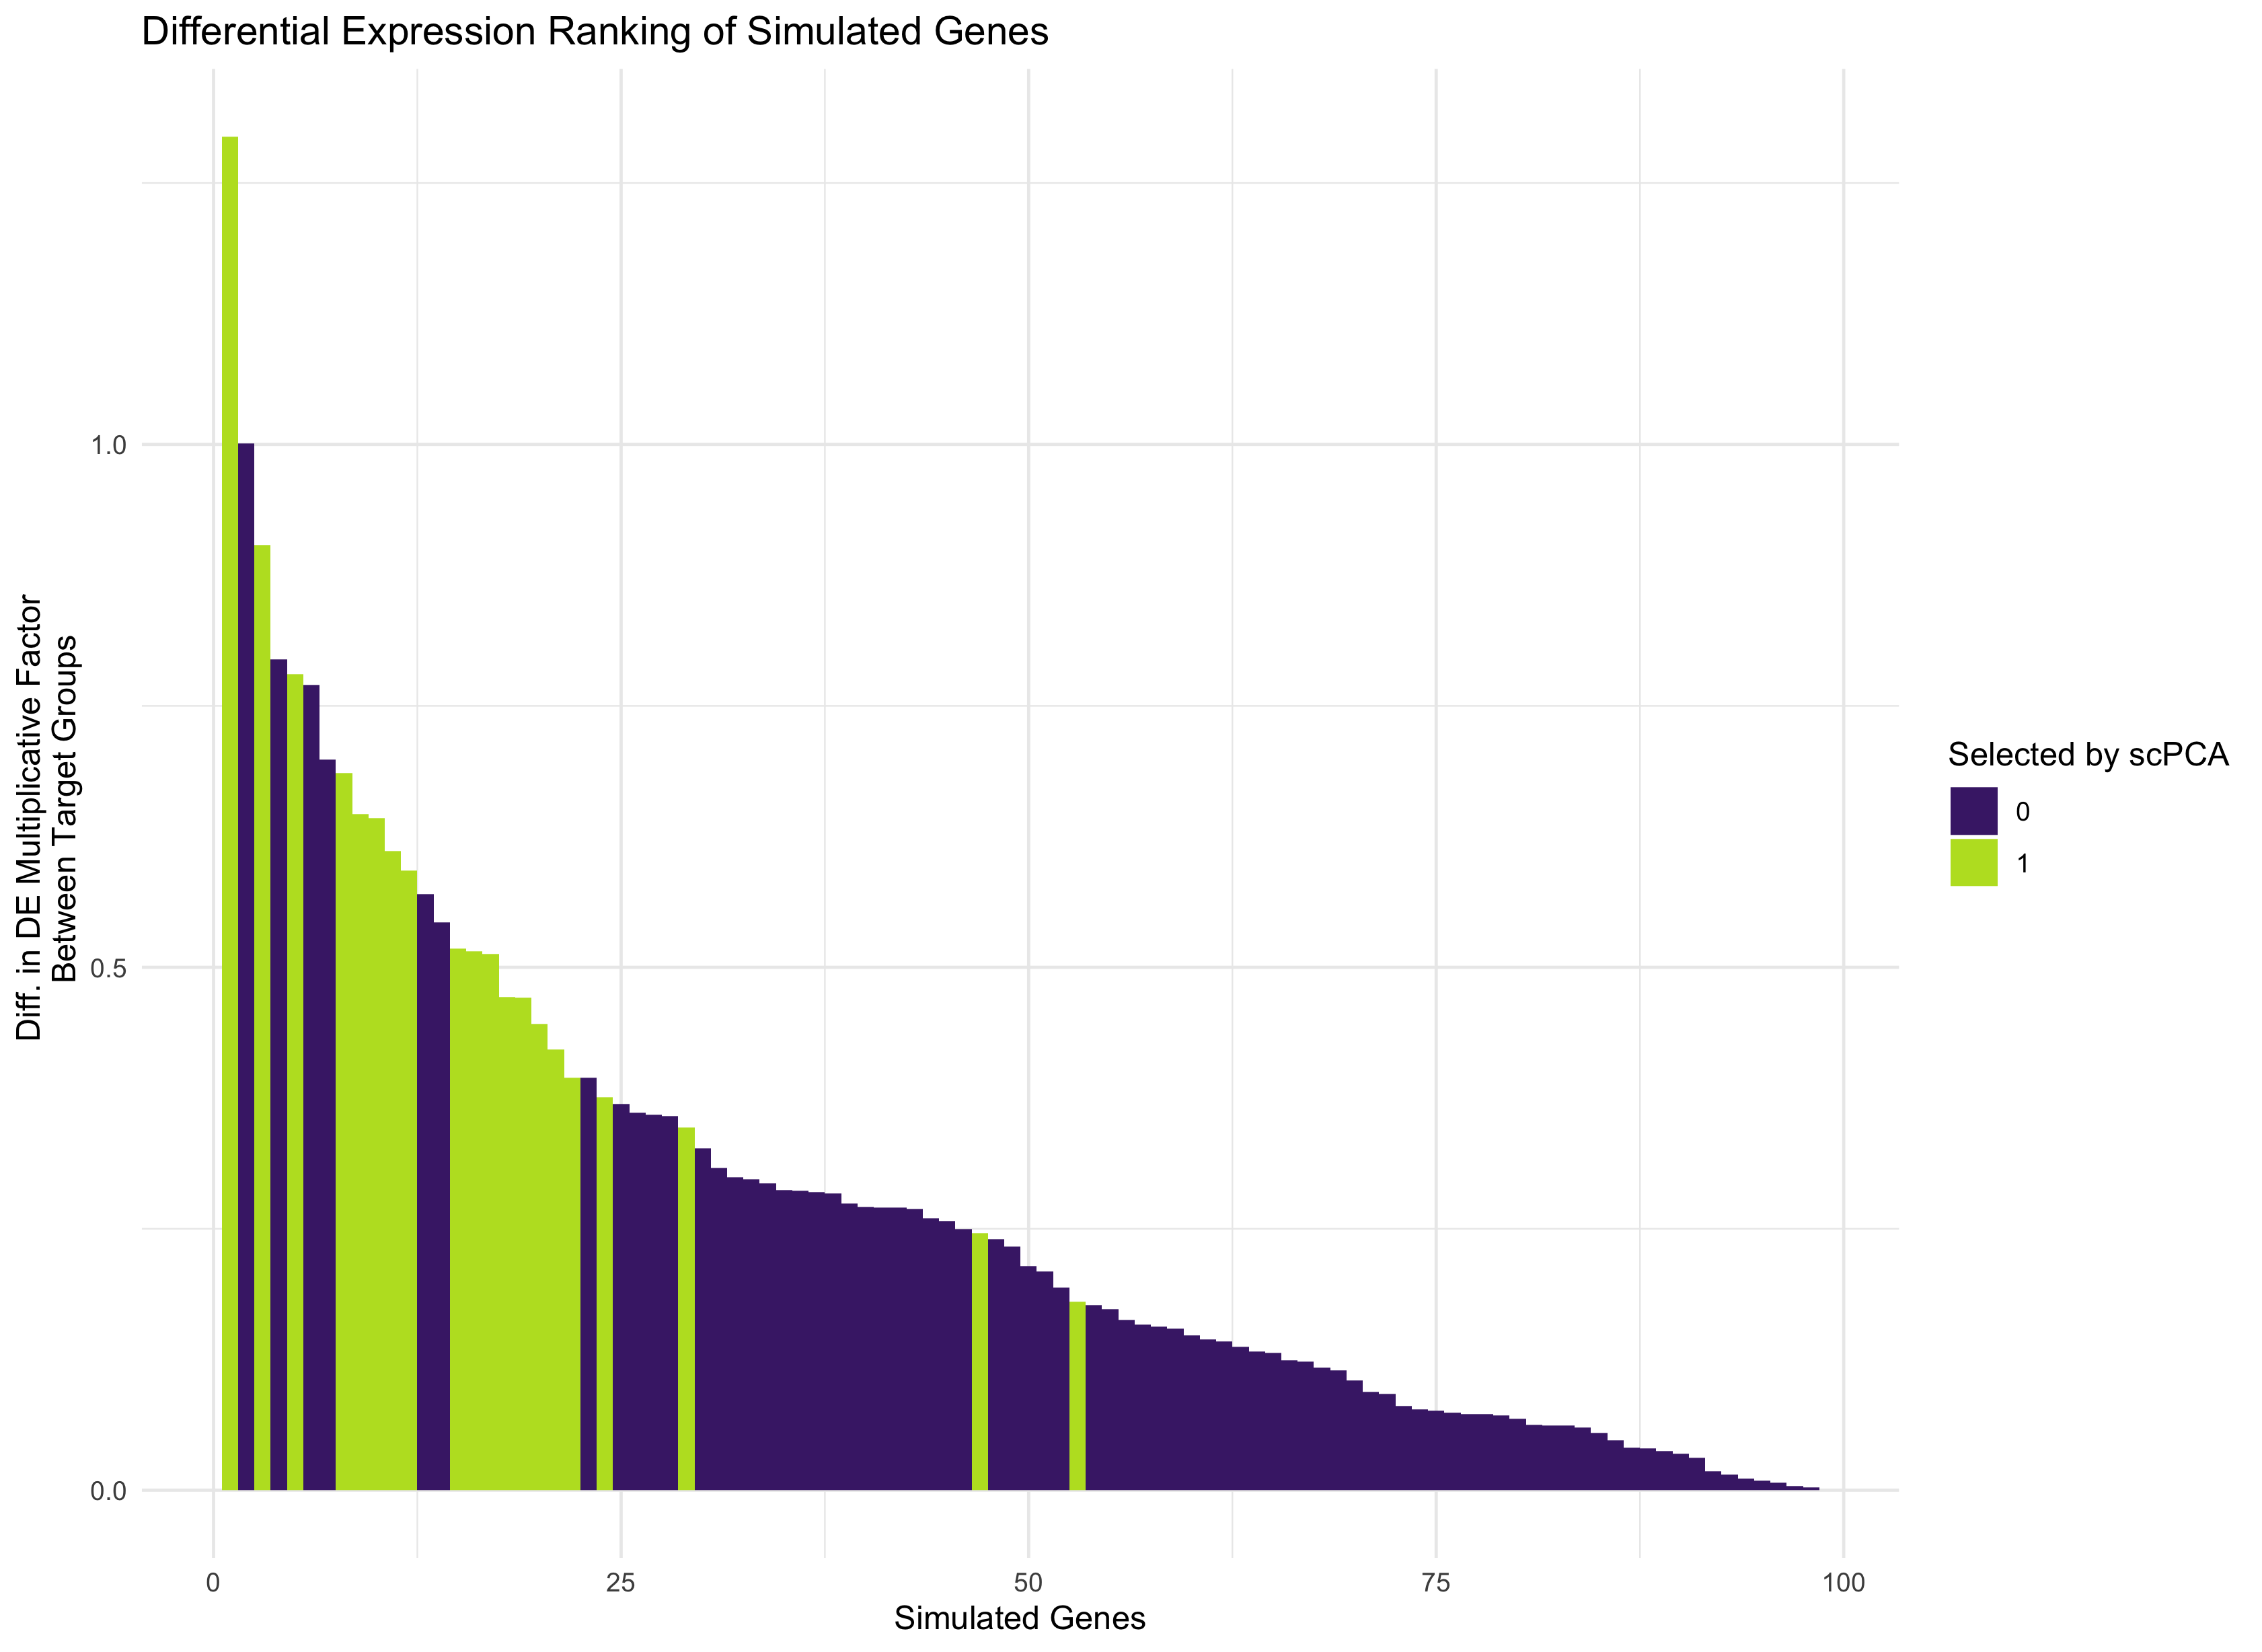
\includegraphics[width=0.9\textwidth]{figures/sim_de_genes}
    \caption{{\em Simulated scRNA-seq data: Differential expression.}
    The 98 differentially expressed genes in the simulated target dataset are ranked in decreasing order of their absolute level of differential expression between groups. In the \textit{Splatter} framework, genes are differentially expressed between groups by way of a group-specific multiplicative factor. Thus, the level of differential expression of any gene between two groups may be computed as the absolute value of the difference between each groups multiplicative factor. We find that all 20 of the genes with non-zero entries in scPCA's first loading vector, highlighted in green, are among the most differentially expressed.}
    \label{fig:sim_de_genes}
\end{figure}

\begin{figure}[!htbp]
    \centering
    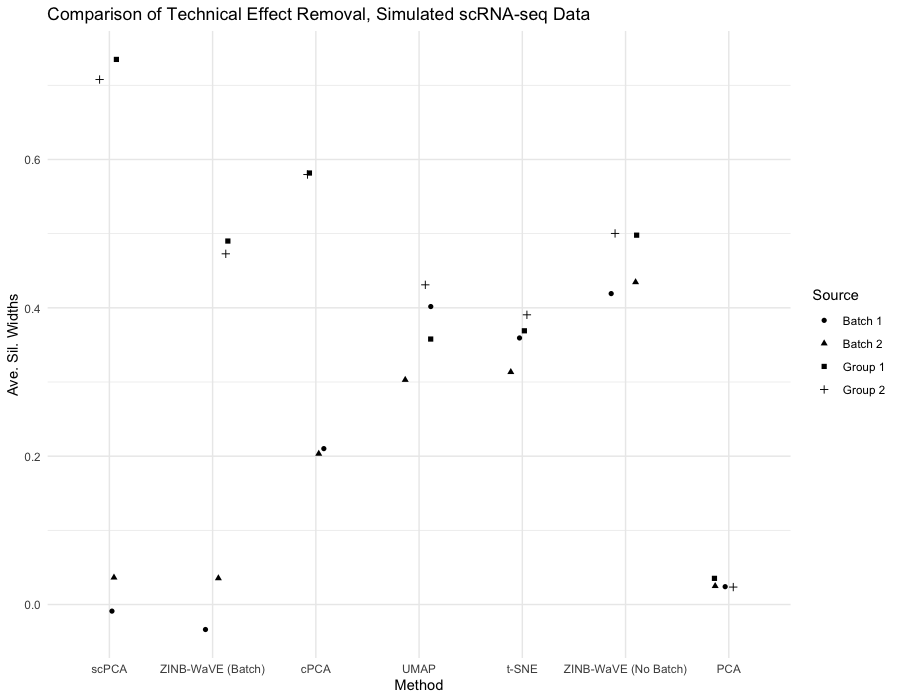
\includegraphics[width=0.9\textwidth]{figures/technical_effect_removal_sim}
    \caption{{\em Simulated scRNA-seq data: Average silhouette width comparison.}
    scPCA produces the densest biological clusters with the least amount of technical noise. The ZINB-WaVE method, when taking into account the batch effect, has a similar performance to scPCA with respect to the removal of unwanted effects, though the biological clusters it produces have lower average silhouette widths. Though cPCA produces denser biological clusters than ZINB-WaVE, it fails to completely remove the batch effect. The remaining methods are unable to disentangle the biological and technical effects. 
    }
    \label{fig:ave_sil_widths}
\end{figure}

\FloatBarrier

\section{Dengue Microarray Data}\label{sup_dengue}

See Section 3.2 %\ref{dengue_data}
for information on the data.

\begin{figure}[!htbp]
    \centering
    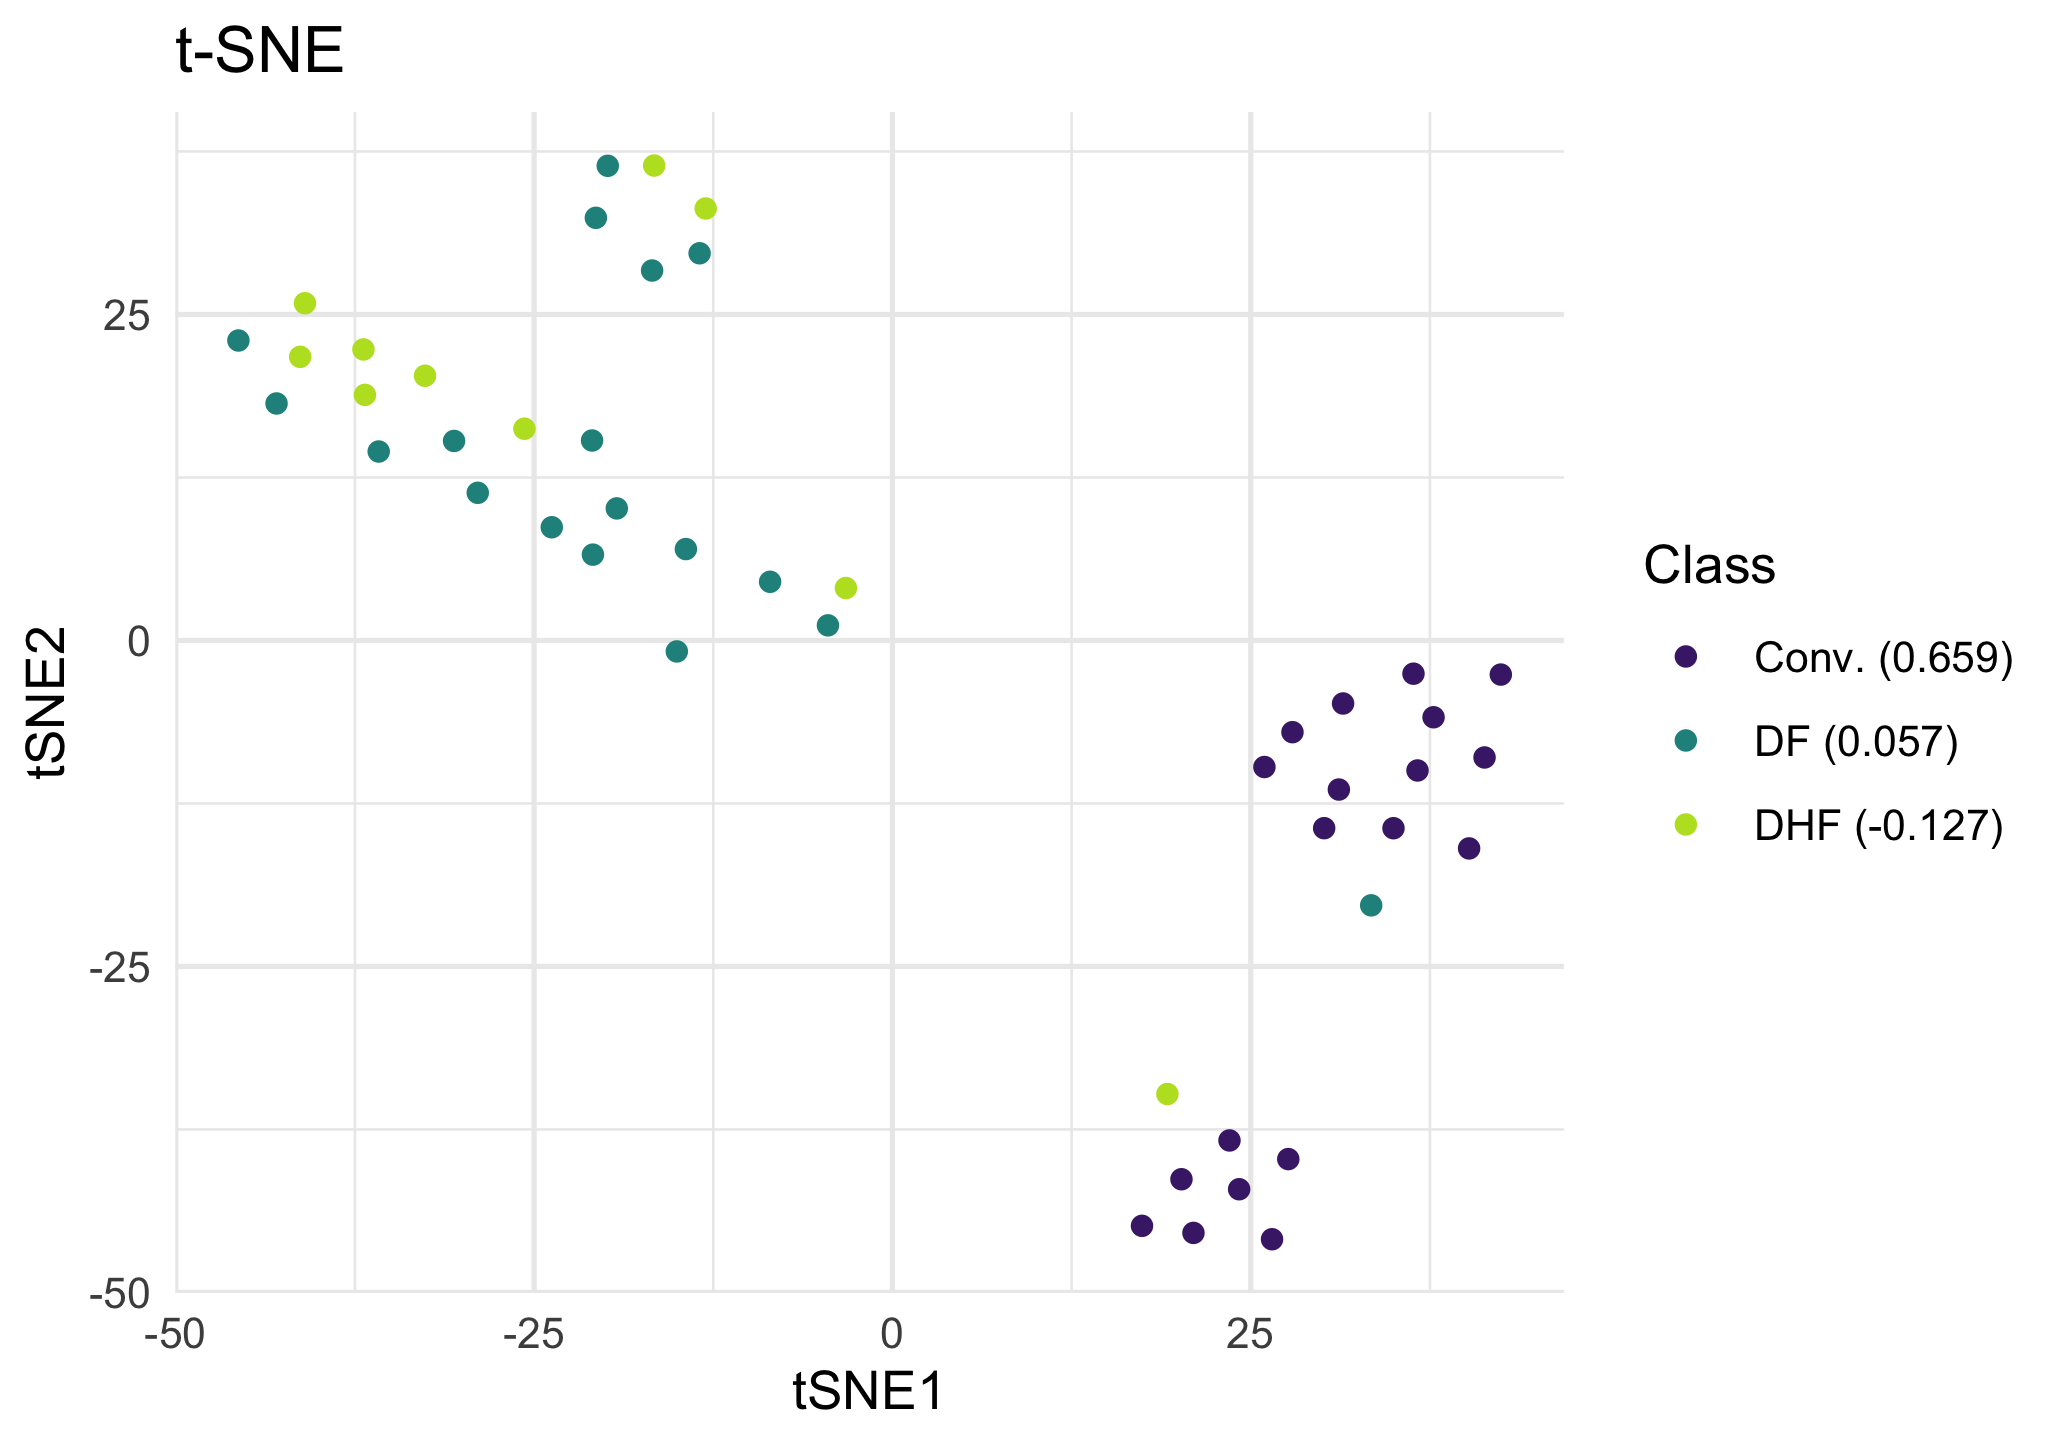
\includegraphics[width=0.5\textwidth]{figures/dengue_tsne}
    \caption{
    {\em Dengue microarray data: t-SNE.}
    Similarly to UMAP, t-SNE almost completely separates the convalescent patients from those with some form of dengue. The two main clusters are further split into distinct sub-clusters, perhaps indicating the presence of a batch effect. 
    }
    \label{fig:dengue_tsne}
\end{figure}

% latex table generated in R 3.6.1 by xtable 1.8-4 package
% Mon Oct 21 14:32:37 2019
\begin{longtable}{| l | p{4cm} | p{8cm} | l |}
  \caption{{\em Dengue microarray data: Genes with non-zero weights in the first scPCA loadings vector.}}
  \label{tab:dengue_1} \\
  \hline
    & Gene Symbol & Gene Name & Weight \\ 
  \hline
  \endhead
  1 & PRSS33 & protease, serine, 33 & -0.0059 \\ 
  2 & PDZK1IP1 & PDZK1 interacting protein 1 & -0.0347 \\ 
  3 & SDC1 & syndecan 1 & 0.2507 \\ 
  4 & CAV1 & caveolin 1, caveolae protein, 22kDa & 0.0889 \\ 
  5 & GGH & gamma-glutamyl hydrolase (conjugase, folylpolygammaglutamyl hydrolase) & 0.2318 \\ 
  6 & PI3 & peptidase inhibitor 3, skin-derived & -0.0209 \\ 
  7 & BUB1B & budding uninhibited by benzimidazoles 1 homolog beta (yeast) & 0.1242 \\ 
  8 & ZWINT & ZW10 interactor & 0.3984 \\ 
  9 & TUBB2A & tubulin, beta 2A & -0.0004 \\ 
  10 & PTGS2 & prostaglandin-endoperoxide synthase 2 (prostaglandin G/H synthase and cyclooxygenase) & -0.0627 \\ 
  11 & TTK & TTK protein kinase & 0.0201 \\ 
  12 & ORM1 /// ORM2 & orosomucoid 1 /// orosomucoid 2 & -0.0055 \\ 
  13 & CD38 & CD38 molecule & 0.0399 \\ 
  14 & CHI3L1 & chitinase 3-like 1 (cartilage glycoprotein-39) & -0.0384 \\ 
  15 & HLA-DQB1 & major histocompatibility complex, class II, DQ beta 1 & 0.0720 \\ 
  16 & BUB1 & budding uninhibited by benzimidazoles 1 homolog (yeast) & 0.0853 \\ 
  17 & CDK1 & cyclin-dependent kinase 1 & 0.2650 \\ 
  18 & IGH@ /// IGHA1 /// IGHA2 /// IGHD /// IGHG1 /// IGHG3 /// IGHG4 /// IGHM /// IGHV4-31 /// LOC100290146 /// LOC100290528 & immunoglobulin heavy locus /// immunoglobulin heavy constant alpha 1 /// immunoglobulin heavy constant alpha 2 (A2m marker) /// immunoglobulin heavy constant delta /// immunoglobulin heavy constant gamma 1 (G1m marker) /// immunoglobulin heavy constant gamma 3 (G3m marker) /// immunoglobulin heavy constant gamma 4 (G4m marker) /// immunoglobulin heavy constant mu /// immunoglobulin heavy variable 4-31 /// hypothetical protein LOC100290146 /// similar to pre-B lymphocyte gene 2 & 0.0180 \\ 
  19 & IGH@ /// IGHA1 /// IGHA2 /// IGHD /// IGHG1 /// IGHG3 /// IGHG4 /// IGHM /// IGHV3-23 /// LOC100126583 /// LOC100290146 /// LOC652128 & immunoglobulin heavy locus /// immunoglobulin heavy constant alpha 1 /// immunoglobulin heavy constant alpha 2 (A2m marker) /// immunoglobulin heavy constant delta /// immunoglobulin heavy constant gamma 1 (G1m marker) /// immunoglobulin heavy constant gamma 3 (G3m marker) /// immunoglobulin heavy constant gamma 4 (G4m marker) /// immunoglobulin heavy constant mu /// immunoglobulin heavy variable 3-23 /// hypothetical LOC100126583 /// hypothetical protein LOC100290146 /// similar to Ig heavy chain V-II region ARH-77 precursor & 0.1867 \\ 
  20 & NOV & nephroblastoma overexpressed gene & -0.0619 \\ 
  21 & SELENBP1 & selenium binding protein 1 & -0.1315 \\ 
  22 & IGHA1 /// IGHG1 /// IGHM /// LOC100290293 & immunoglobulin heavy constant alpha 1 /// immunoglobulin heavy constant gamma 1 (G1m marker) /// immunoglobulin heavy constant mu /// similar to hCG2042717 & 0.0162 \\ 
  23 & CEP55 & centrosomal protein 55kDa & 0.2863 \\ 
  24 & PBK & PDZ binding kinase & 0.1358 \\ 
  25 & SHCBP1 & SHC SH2-domain binding protein 1 & 0.2901 \\ 
  26 & MGC29506 & plasma cell-induced ER protein 1 & 0.4012 \\ 
  27 & CNTNAP3 & contactin associated protein-like 3 & -0.0494 \\ 
  28 & JAZF1 & JAZF zinc finger 1 & -0.0441 \\ 
  29 & KIAA1324 & KIAA1324 & -0.0962 \\ 
  30 & CDCA2 & cell division cycle associated 2 & 0.3858 \\ 
  31 & KLHL14 & kelch-like 14 (Drosophila) & 0.0801 \\ 
  32 & CYAT1 & cyclosporin A transporter 1 & 0.1657 \\ 
  33 & HLA-DRB1 /// HLA-DRB3 /// HLA-DRB4 /// HLA-DRB5 /// LOC100294036 & major histocompatibility complex, class II, DR beta 1 /// major histocompatibility complex, class II, DR beta 3 /// major histocompatibility complex, class II, DR beta 4 /// major histocompatibility complex, class II, DR beta 5 /// similar to HLA class II histocompatibility antigen, DRB1-7 beta chain & 0.0422 \\ 
  34 & FLJ10357 & protein SOLO & -0.0966 \\ 
   \hline
\end{longtable}

% latex table generated in R 3.6.1 by xtable 1.8-4 package
% Mon Oct 21 14:52:46 2019
\begin{longtable}{| l | p{4cm} | p{8cm} | l |}
  \caption{{\em Dengue microarray data: Genes with non-zero weights in the second scPCA loadings vector.}}  \label{tab:dengue_2} \\
  \hline
 & Gene Symbol & Gene Name & Weight \\ 
  \hline
  \endhead
  1 & PRSS33 & protease, serine, 33 & 0.1822 \\ 
  2 & IFI27 & interferon, alpha-inducible protein 27 & -0.0147 \\ 
  3 & PI3 & peptidase inhibitor 3, skin-derived & 0.1692 \\ 
  4 & SLC2A5 & solute carrier family 2 (facilitated glucose/fructose transporter), member 5 & 0.0701 \\ 
  5 & MYOM2 & myomesin (M-protein) 2, 165kDa & -0.0278 \\ 
  6 & HLA-DRB4 & major histocompatibility complex, class II, DR beta 4 & -0.0620 \\ 
  7 & IGH@ /// IGHA1 /// IGHD /// IGHG1 /// IGHG3 /// IGHG4 /// IGHM /// IGHV3-23 /// IGHV4-31 /// LOC100290146 /// LOC100290528 & immunoglobulin heavy locus /// immunoglobulin heavy constant alpha 1 /// immunoglobulin heavy constant delta /// immunoglobulin heavy constant gamma 1 (G1m marker) /// immunoglobulin heavy constant gamma 3 (G3m marker) /// immunoglobulin heavy constant gamma 4 (G4m marker) /// immunoglobulin heavy constant mu /// immunoglobulin heavy variable 3-23 /// immunoglobulin heavy variable 4-31 /// hypothetical protein LOC100290146 /// similar to pre-B lymphocyte gene 2 & 0.4987 \\ 
  8 & IGKV3-20 & Immunoglobulin kappa variable 3-20 & 0.1623 \\ 
  9 & RSAD2 & radical S-adenosyl methionine domain containing 2 & -0.2294 \\ 
  10 & USP18 & ubiquitin specific peptidase 18 & -0.4599 \\ 
  11 & SIGLEC1 & sialic acid binding Ig-like lectin 1, sialoadhesin & -0.2750 \\ 
  12 & KCTD14 & potassium channel tetramerisation domain containing 14 & -0.3142 \\ 
  13 & FAM118A & family with sequence similarity 118, member A & -0.1382 \\ 
  14 &  &  & 0.0269 \\ 
  15 & SLC16A14 & solute carrier family 16, member 14 (monocarboxylic acid transporter 14) & 0.3232 \\ 
  16 & ANKRD22 & ankyrin repeat domain 22 & -0.2800 \\ 
  17 & KLC3 & kinesin light chain 3 & 0.1021 \\ 
  18 & SIGLEC1 & sialic acid binding Ig-like lectin 1, sialoadhesin & -0.0434 \\ 
   \hline
\end{longtable}

\begin{figure}[!htbp]
    \centering
    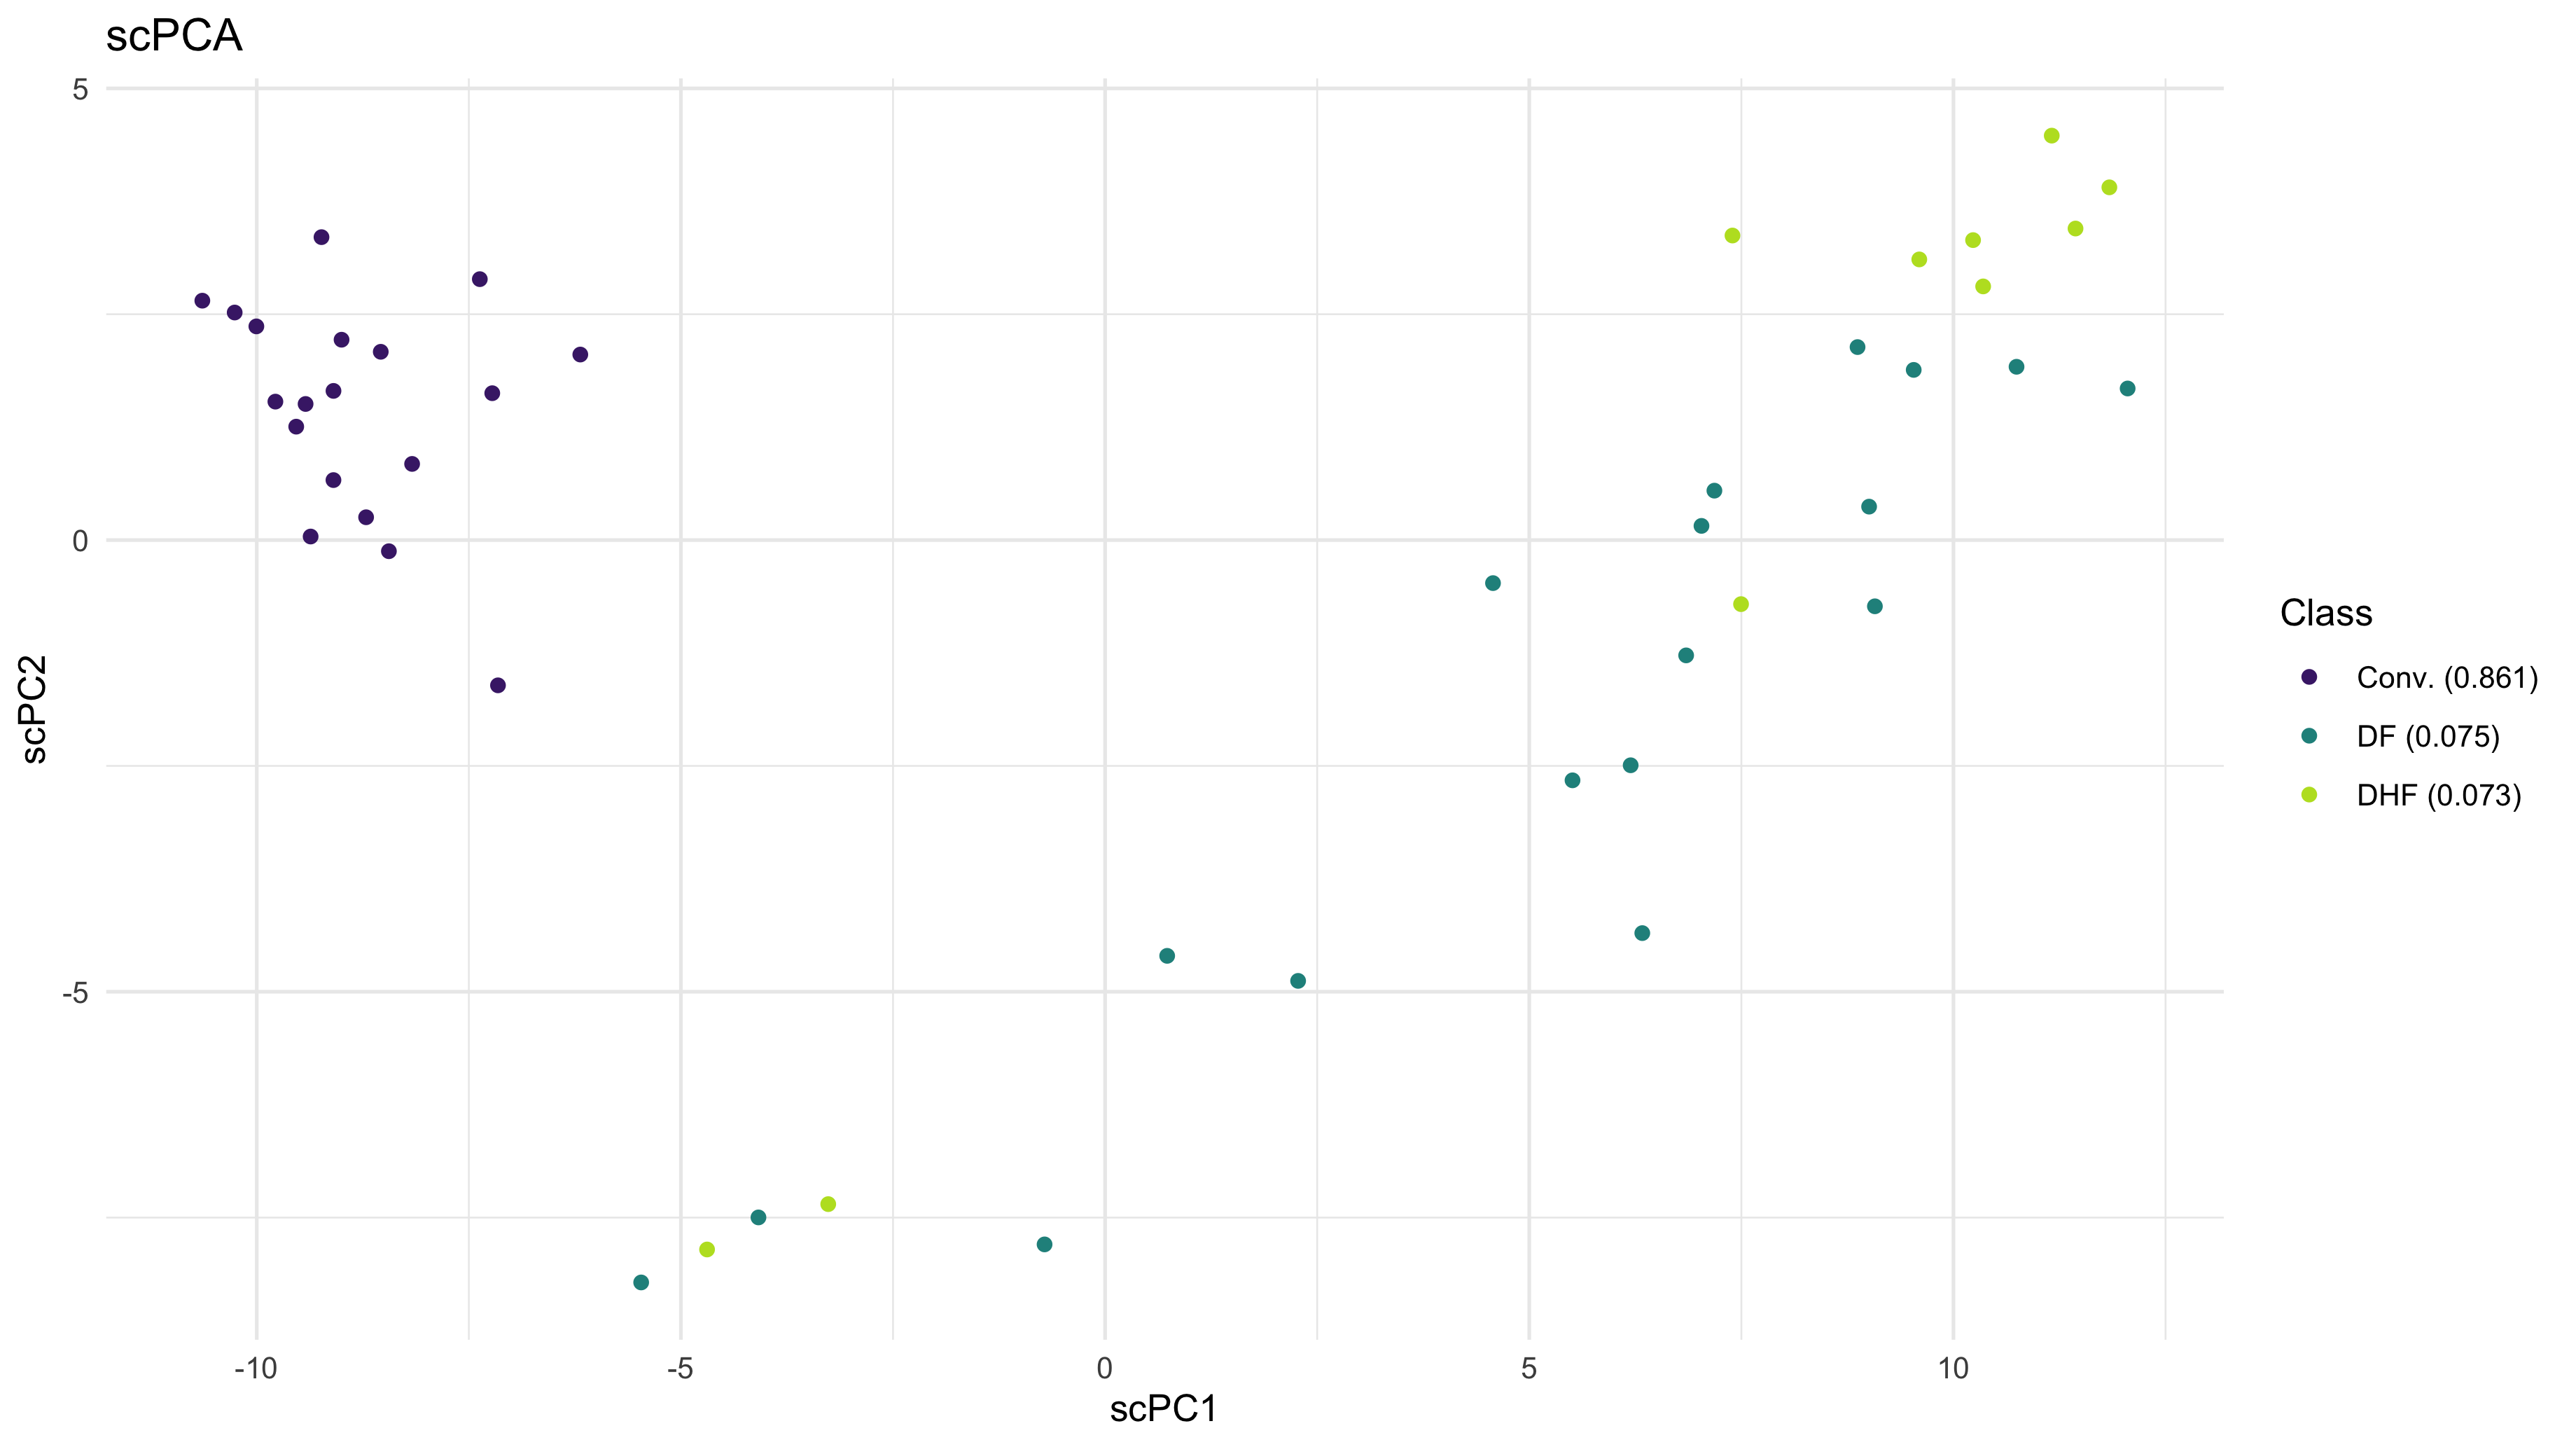
\includegraphics[width=0.9\textwidth]{figures/dengue_cpca_centers}
    \caption{
    {\em Dengue microarray data: cPCA.}
    When varying the \textit{a priori} specified number of clusters for cPCA, all four embeddings are virtually identical, suggesting that optimal contrastive parameters were selected in each case. Thus, cPCA is robust to misspecifications of the number of clusters.}
    \label{fig:dengue_cpca_centers}
\end{figure}

\begin{figure}[!htbp]
    \centering
    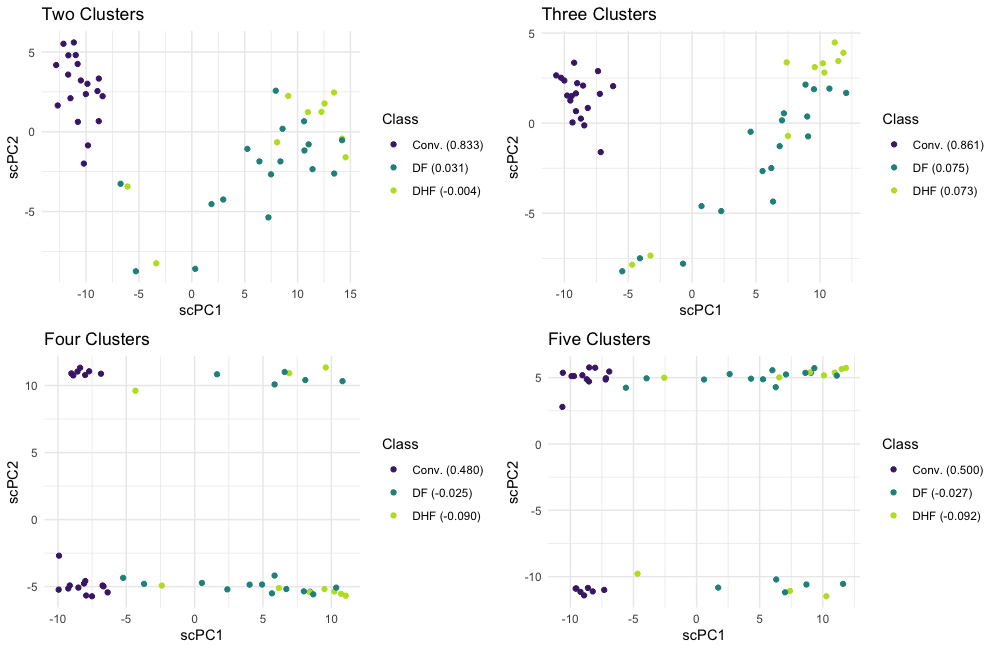
\includegraphics[width=0.9\textwidth]{figures/dengue_scpca_centers}
    \caption{
    {\em Dengue microarray data: scPCA.}
    When varying the \textit{a priori} specified number of clusters for scPCA, we find that the two-dimensional embeddings are sensitive to this choice. When scPCA is performed on this data with four and five clusters, the results resemble those produced by PCA.}
    \label{fig:dengue_scpca_centers}
\end{figure}

\FloatBarrier

\newpage

\section{Leukemia Patient scRNA-seq Data}

See Section 3.3 %\ref{leukemia_data}
for information on the data.

\begin{figure}[!htbp]
  \centering
  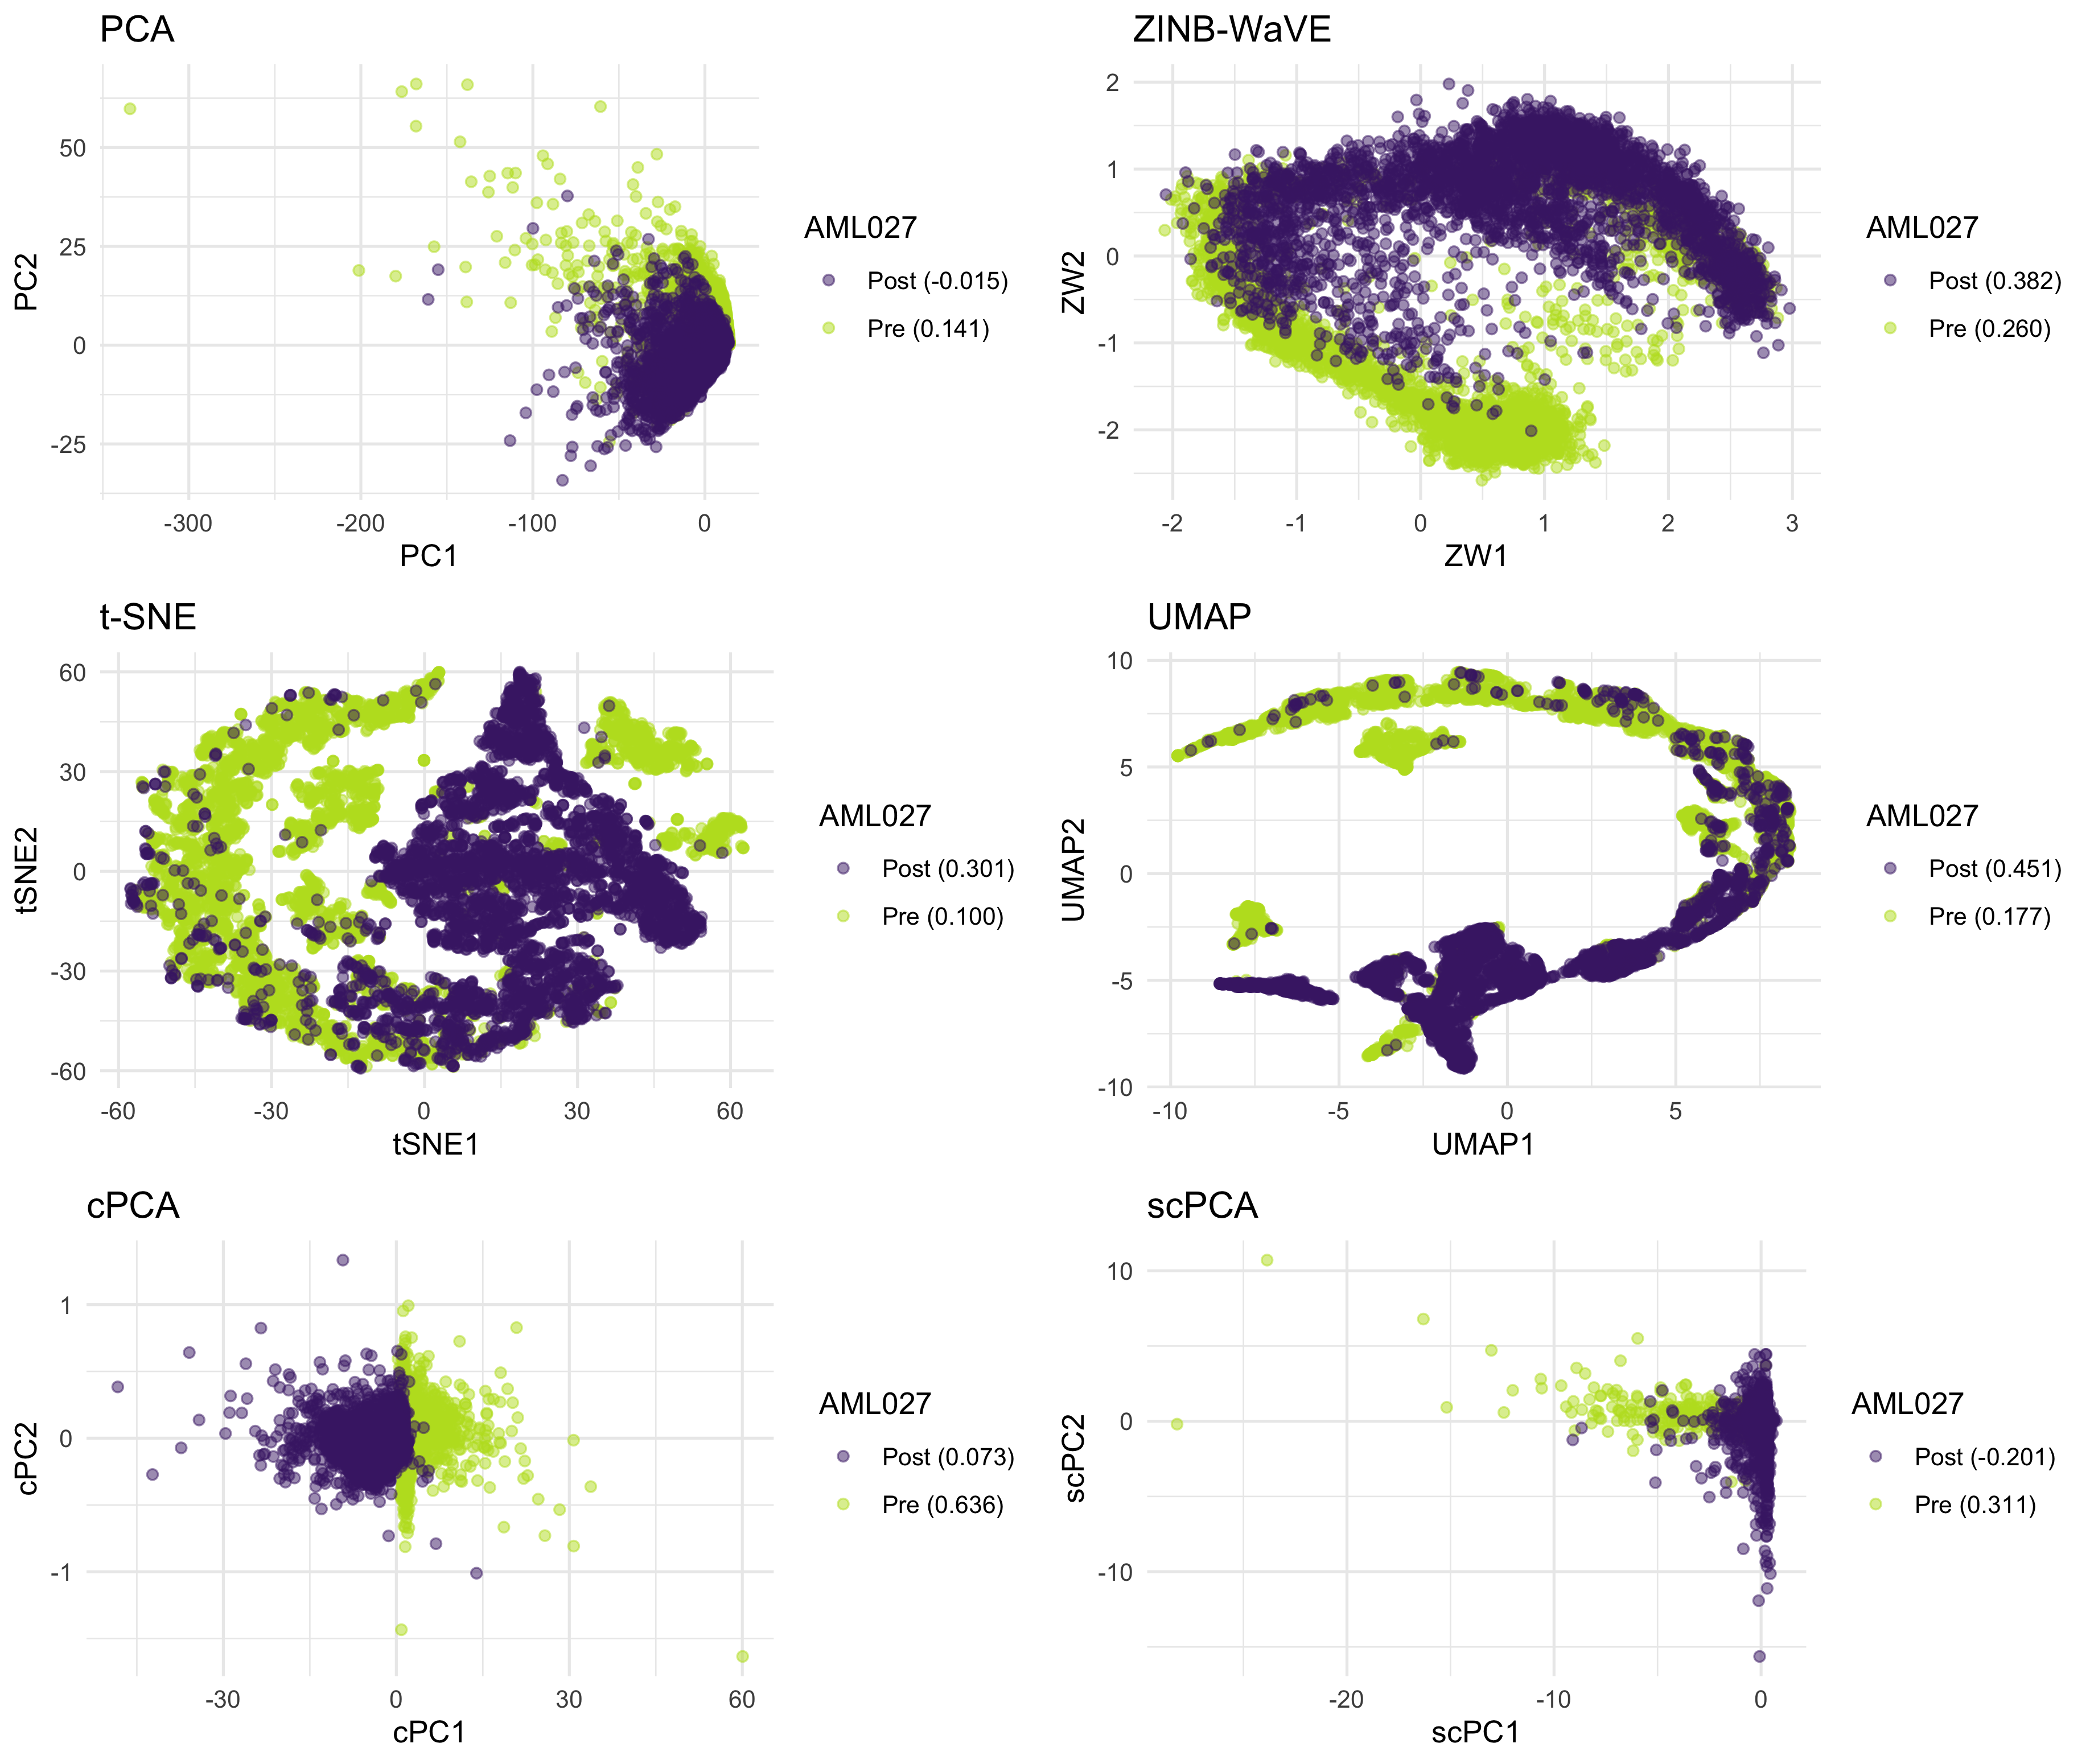
\includegraphics[width=0.9\textwidth]{figures/aml027_results}
  \caption{
  {\em AML Patient 027 scRNA-seq data.} The two-dimensional embeddings of the patient's BMMC cells produced by PCA, ZINB-WaVE, t-SNE, UMAP, cPCA, and scPCA. cPCA and scPCA produce two-dimensional representations that distinguish between the pre- and post-transplant cells of Patient 027. Although cPCA's embedding contains denser clusters, scPCA's clusters are more distinct --- though they are oddly shaped. This is the result of sparsity: the scPCA embedding is produced with the count data of only three genes.}
  \label{fig:comp_leuk_pat2}
\end{figure}
\FloatBarrier

\section{Mouse Protein Expression Data}\label{sup_mice}

Down Syndrome, the leading genetic cause of intellectual disability \citeSM{Irving2008}, is the result of trisomy of all or part of the long arm of chromosome 21 \citeSM{Ahmed2015}. Recently, researchers have begun exploring the use of pharmacotherapies to mitigate these cognitive deficits using the Ts65Dn mouse model \citeSM{Ahmed2015,Higuera2015}. Though not a perfect model for the study of Down Syndrome, the Ts65Dn displays many relevant neurological phenotypic features, such as deficits in learning and memory \citeSM{Rueda2012}.

Ahmed et al. \citeSM{Ahmed2015} analyzed protein expression in the hippocampus and cortex of Ts65Dn and control mice after exposure to context fear conditioning and Memantine treatment. Memantine, a drug often prescribed to Alzheimer's patients, has been demonstrated to improve performance of the Ts65Dn in tasks that reflect cognitive abilities \citeSM{Ahmed2015}. The corresponding dataset was made available by Higuera et al. \citeSM{Higuera2015}. The data consist of normalized expression measures for 77 proteins from subcellular fractions of the cortex assayed from 38 control and 34 Ts65Dn mice. Each protein expression measurement was repeated 15 times (i.e., 15 technical replicates per mouse for each of the 77 proteins), though a small number of replicates contain missing protein expression measurements due to technical artifacts \citeSM{Higuera2015}. More details on the experimental design are provided in fig. \ref{fig:exp_design}.

\begin{figure}[!htbp]
    \centering
    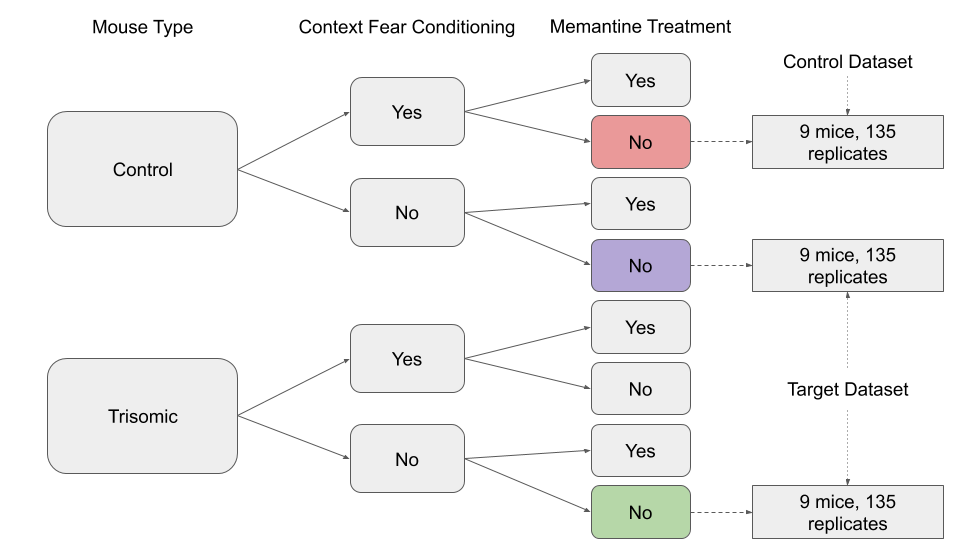
\includegraphics[width=0.9\textwidth]{figures/mice_exp_design}
    \caption{
    {\em Mouse protein expression data: Experimental design.} 
    The control dataset is comprised of protein expression measurements for 15 technical replicates from each of 9 control mice subject to context fear conditioning and given a placebo (red leaf). The target dataset consists of protein expression measurements for 15 technical replicates from each of 9 control mice not subject to context fear condition and given a placebo (purple leaf) and 15 technical replicates from each of 9 trisomic mice not subject to context fear condition and given a placebo (green leaf).}
    \label{fig:exp_design}
\end{figure}

To demonstrate scPCA's capacity to capture biologically meaningful and interpretable variation in protein expression data, the technical replicates of the subset comprising 9 control and 9 Ts65Dn mice not subject to context fear conditioning and given a placebo were designated as the target dataset. The technical replicates of the subset of 9 control mice that were subject to context fear conditioning and given a placebo made up the background dataset, as the variation in their protein expression measurements are believed to be similar to that found in the control mice of the target dataset. The data are identical to those used by Abid et al. \citeSM{Abid2018} to demonstrate cPCA. PCA, t-SNE, UMAP, cPCA, and scPCA were applied to the target dataset (fig.~\ref{fig:comp_mice}A) to identify differences in protein expression between the control and trisomic mice not exposed to the context fear conditioning experiment. In addition to the target dataset, cPCA and scPCA took as input the column-centered background dataset and specified two clusters \textit{a priori}. The embedding produced by t-SNE is substantially worse than other methods because it generates spurious sub-clusters (fig.~\ref{fig:mice_tsne}).

PCA proved incapable of distinguishing between the biological groups of interest. UMAP, cPCA, and scPCA successfully split the control and trisomic mice into virtually distinct clusters, though the number of clusters found by UMAP and cPCA in two dimensions did not match, even when varying the \textit{a priori} specified number of clusters in cPCA (fig.~\ref{fig:mice_cpca_centers}). Comparing the results of UMAP and scPCA, we find that they produce the same number of clusters, but their representations of the global structure are markedly different, even when varying the number of clusters specified \textit{a priori} in scPCA (fig.~\ref{fig:mice_scpca_centers}). The presence of distinct Ts65Dn clusters in UMAP's representation may correspond to technical noise that is diminished in cPCA's and scPCA's embeddings, or may arise from UMAP's inability to dependably capture global structure. We also remark that cPCA and scPCA produce very similar embeddings, up to a rotation; however, the first and second columns of scPCA's loadings matrix contain merely 12 and 16 non-zero entries, respectively (fig.~\ref{fig:comp_mice}B). Also note that the the separation of control and trisomic mice by scPCA only occurs in scPC2: the proteins with non-zero weights in its corresponding loading vector include AKT, APP, SOD1, and GSK3, each of which has been associated with Down Syndrome in human or mouse models \citeSM{Troca-Marn9445,Niceta2015,Gulesserian2001,Isacson2002}.  The full list of proteins with non-zero weights in the first two loadings vectors of scPCA are provided in Table \ref{tab:mouse_prot_1} and  Table \ref{tab:mouse_prot_2}.

\begin{figure}[!htbp]
  \centering
  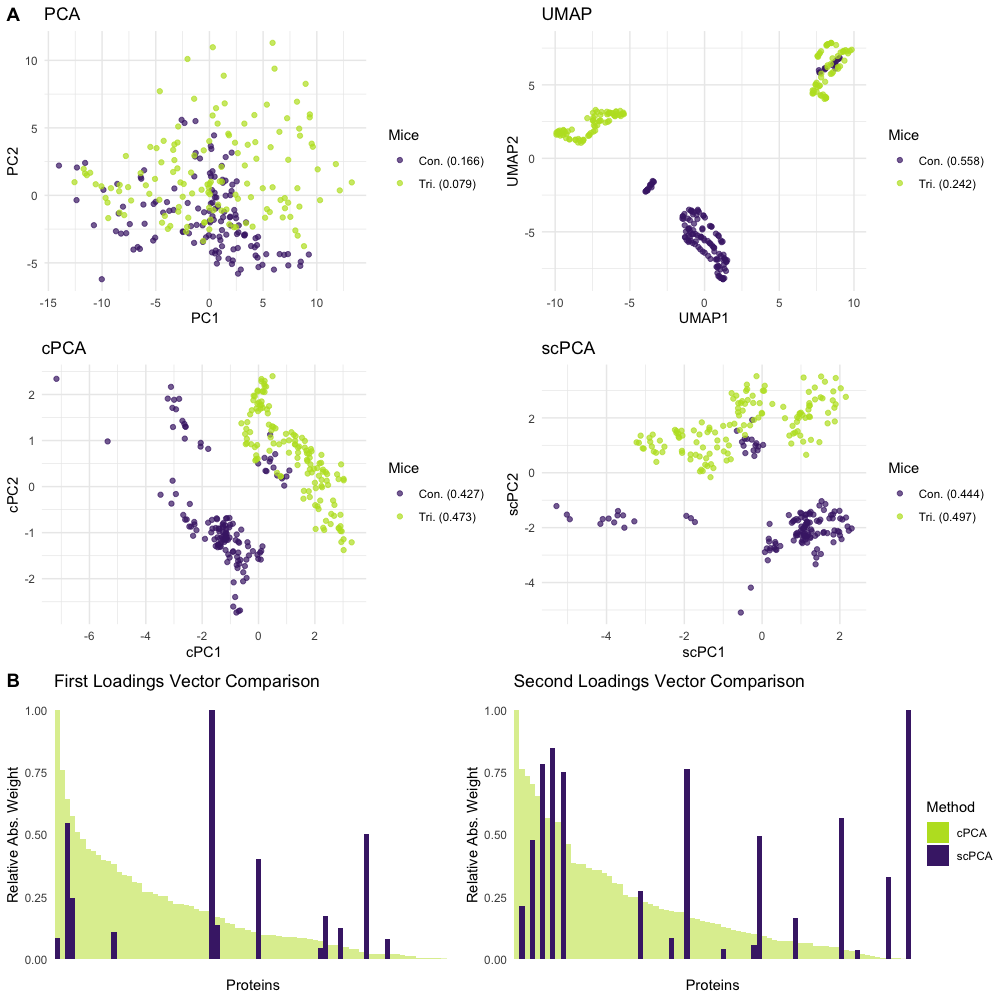
\includegraphics[width=0.9\textwidth]{figures/mice_results}
  \caption{{\em Mouse protein expression data.} \textbf{A} All methods but PCA were capable of separating the control from the trisomic mice, though it is unclear why UMAP splits the Ts65Dn mice into two distinct groups. scPCA's low-dimensional representation of the protein expression data is markedly similar to that of cPCA, up to a rotation, despite relying on only a fraction of non-zero values in the loadings matrix. On average, scPCA also produces the tightest clusters. Note: a small group of control mice were clustered with the trisomic mice in the UMAP, cPCA, and scPCA representation, potentially comprising a group of mislabeled mice. \textbf{B} scPCA's leading vectors of loadings are much sparser than those of cPCA, increasing the interpretability of findings and clarity of the visualization. The differing rotations of cPCA and scPCA, in addition to the drastically different weighting scheme of the proteins in their respective loadings matrices, may indicate that the contrastive step performed by cPCA does not sufficiently dampen spurious sources of variation in the data.}
  \label{fig:comp_mice}
\end{figure}

\begin{figure}[!htbp]
    \centering
    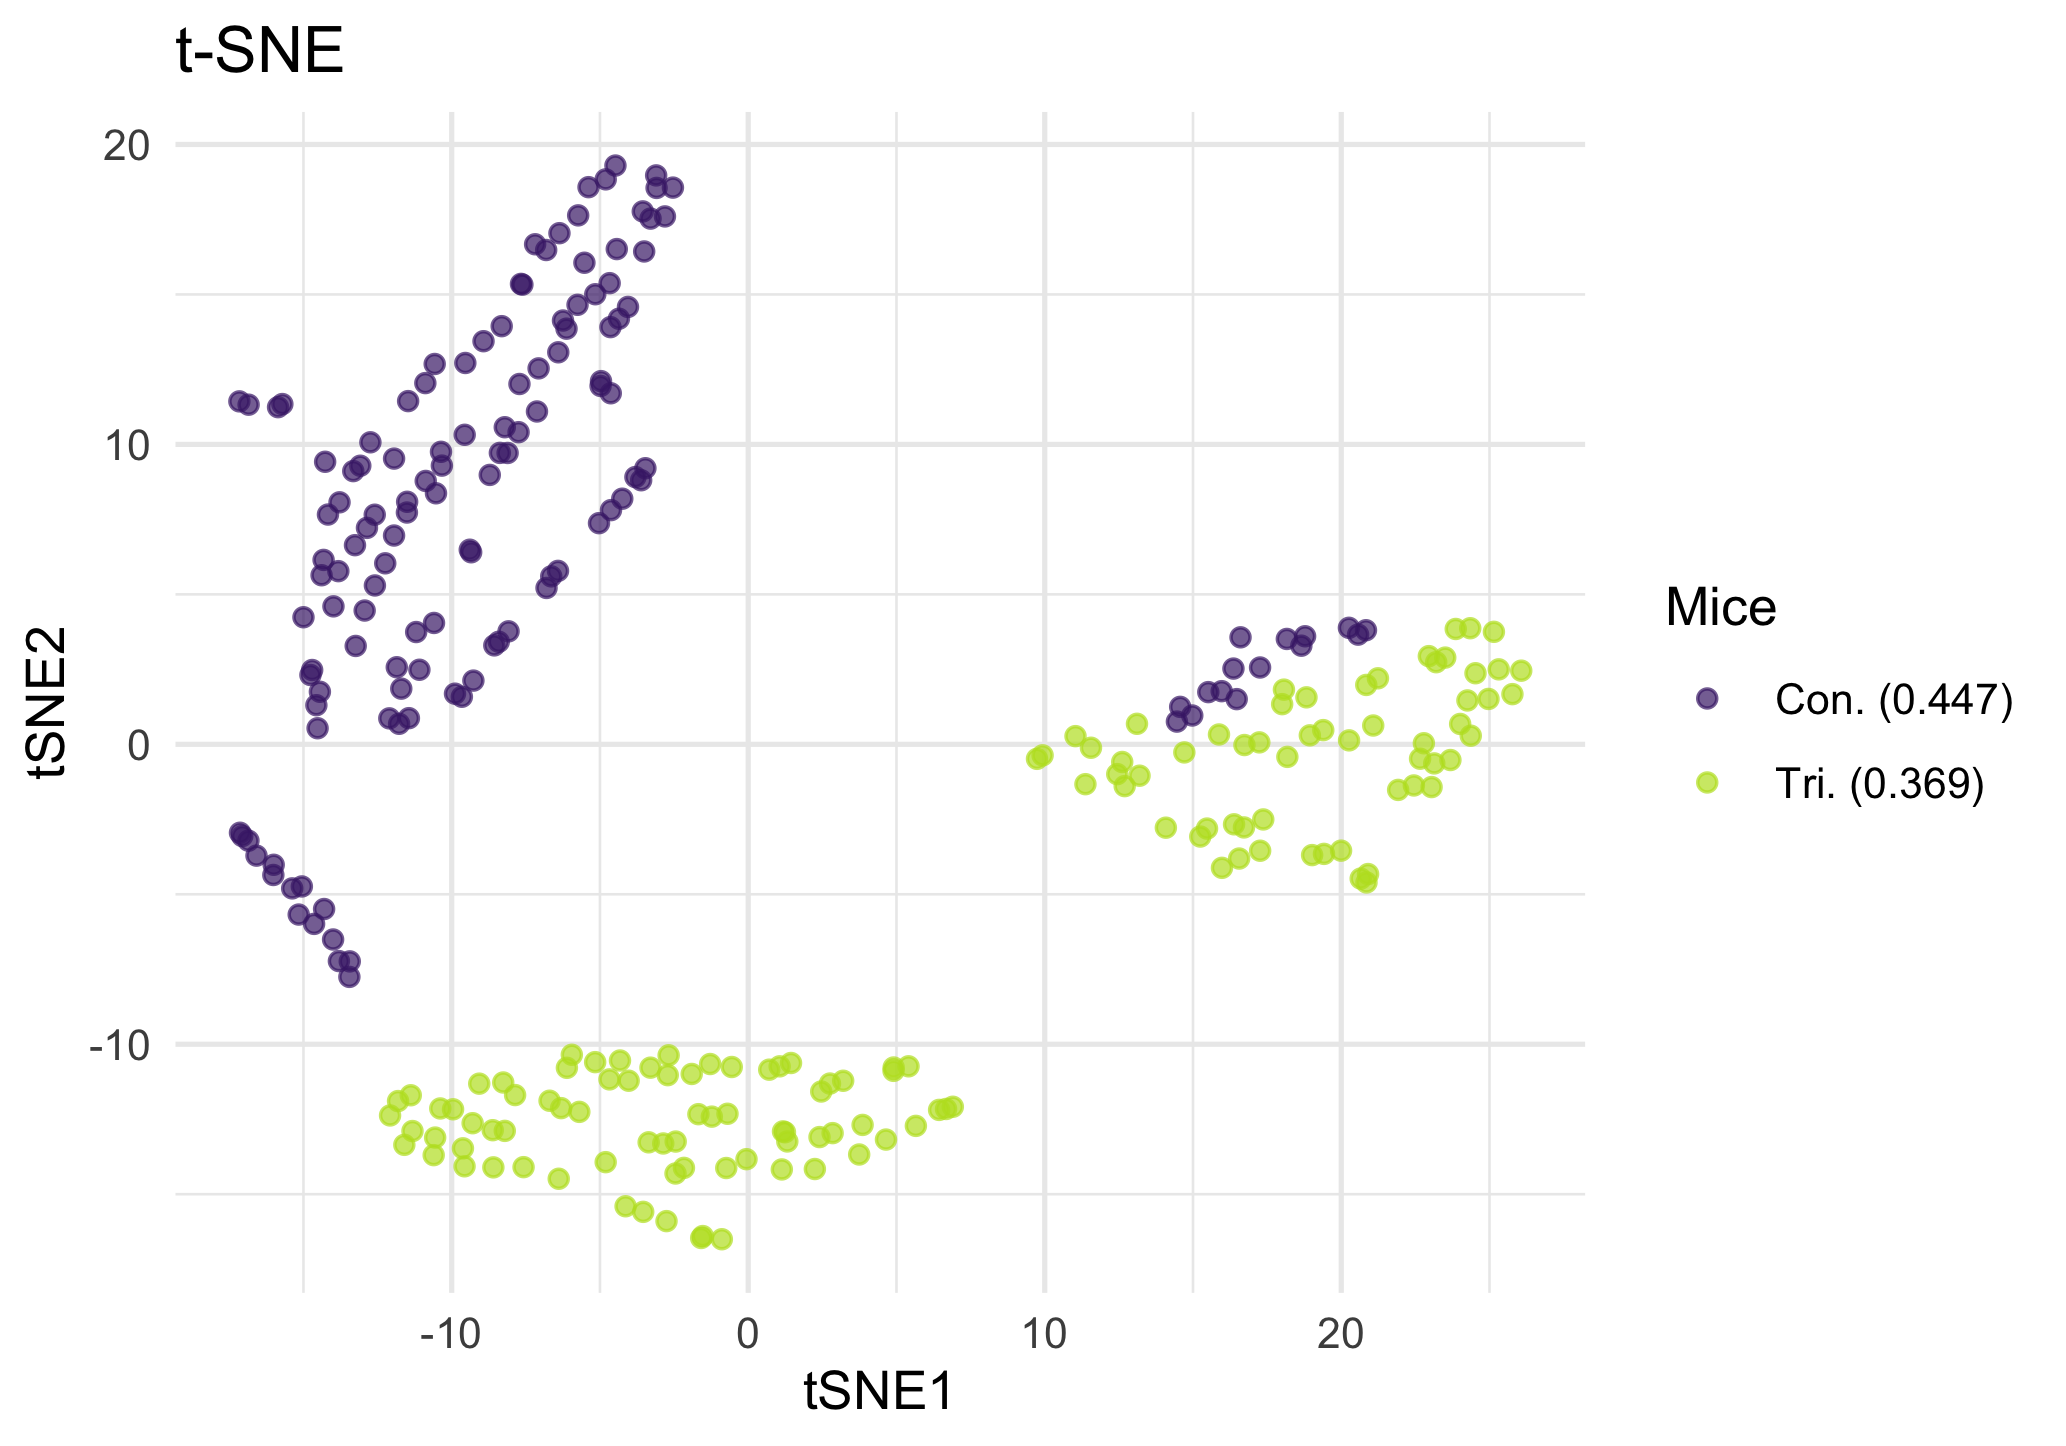
\includegraphics[width=0.5\textwidth]{figures/mice_tsne}
    \caption{
    \textit{Mouse protein expression data: t-SNE.}
    t-SNE produces almost linearly-separable clusters, though these clusters contain many fractured, spurious sub-clusters that do not relate to biological signal.
    }
    \label{fig:mice_tsne}
\end{figure}

\begin{figure}[!htbp]
    \centering
    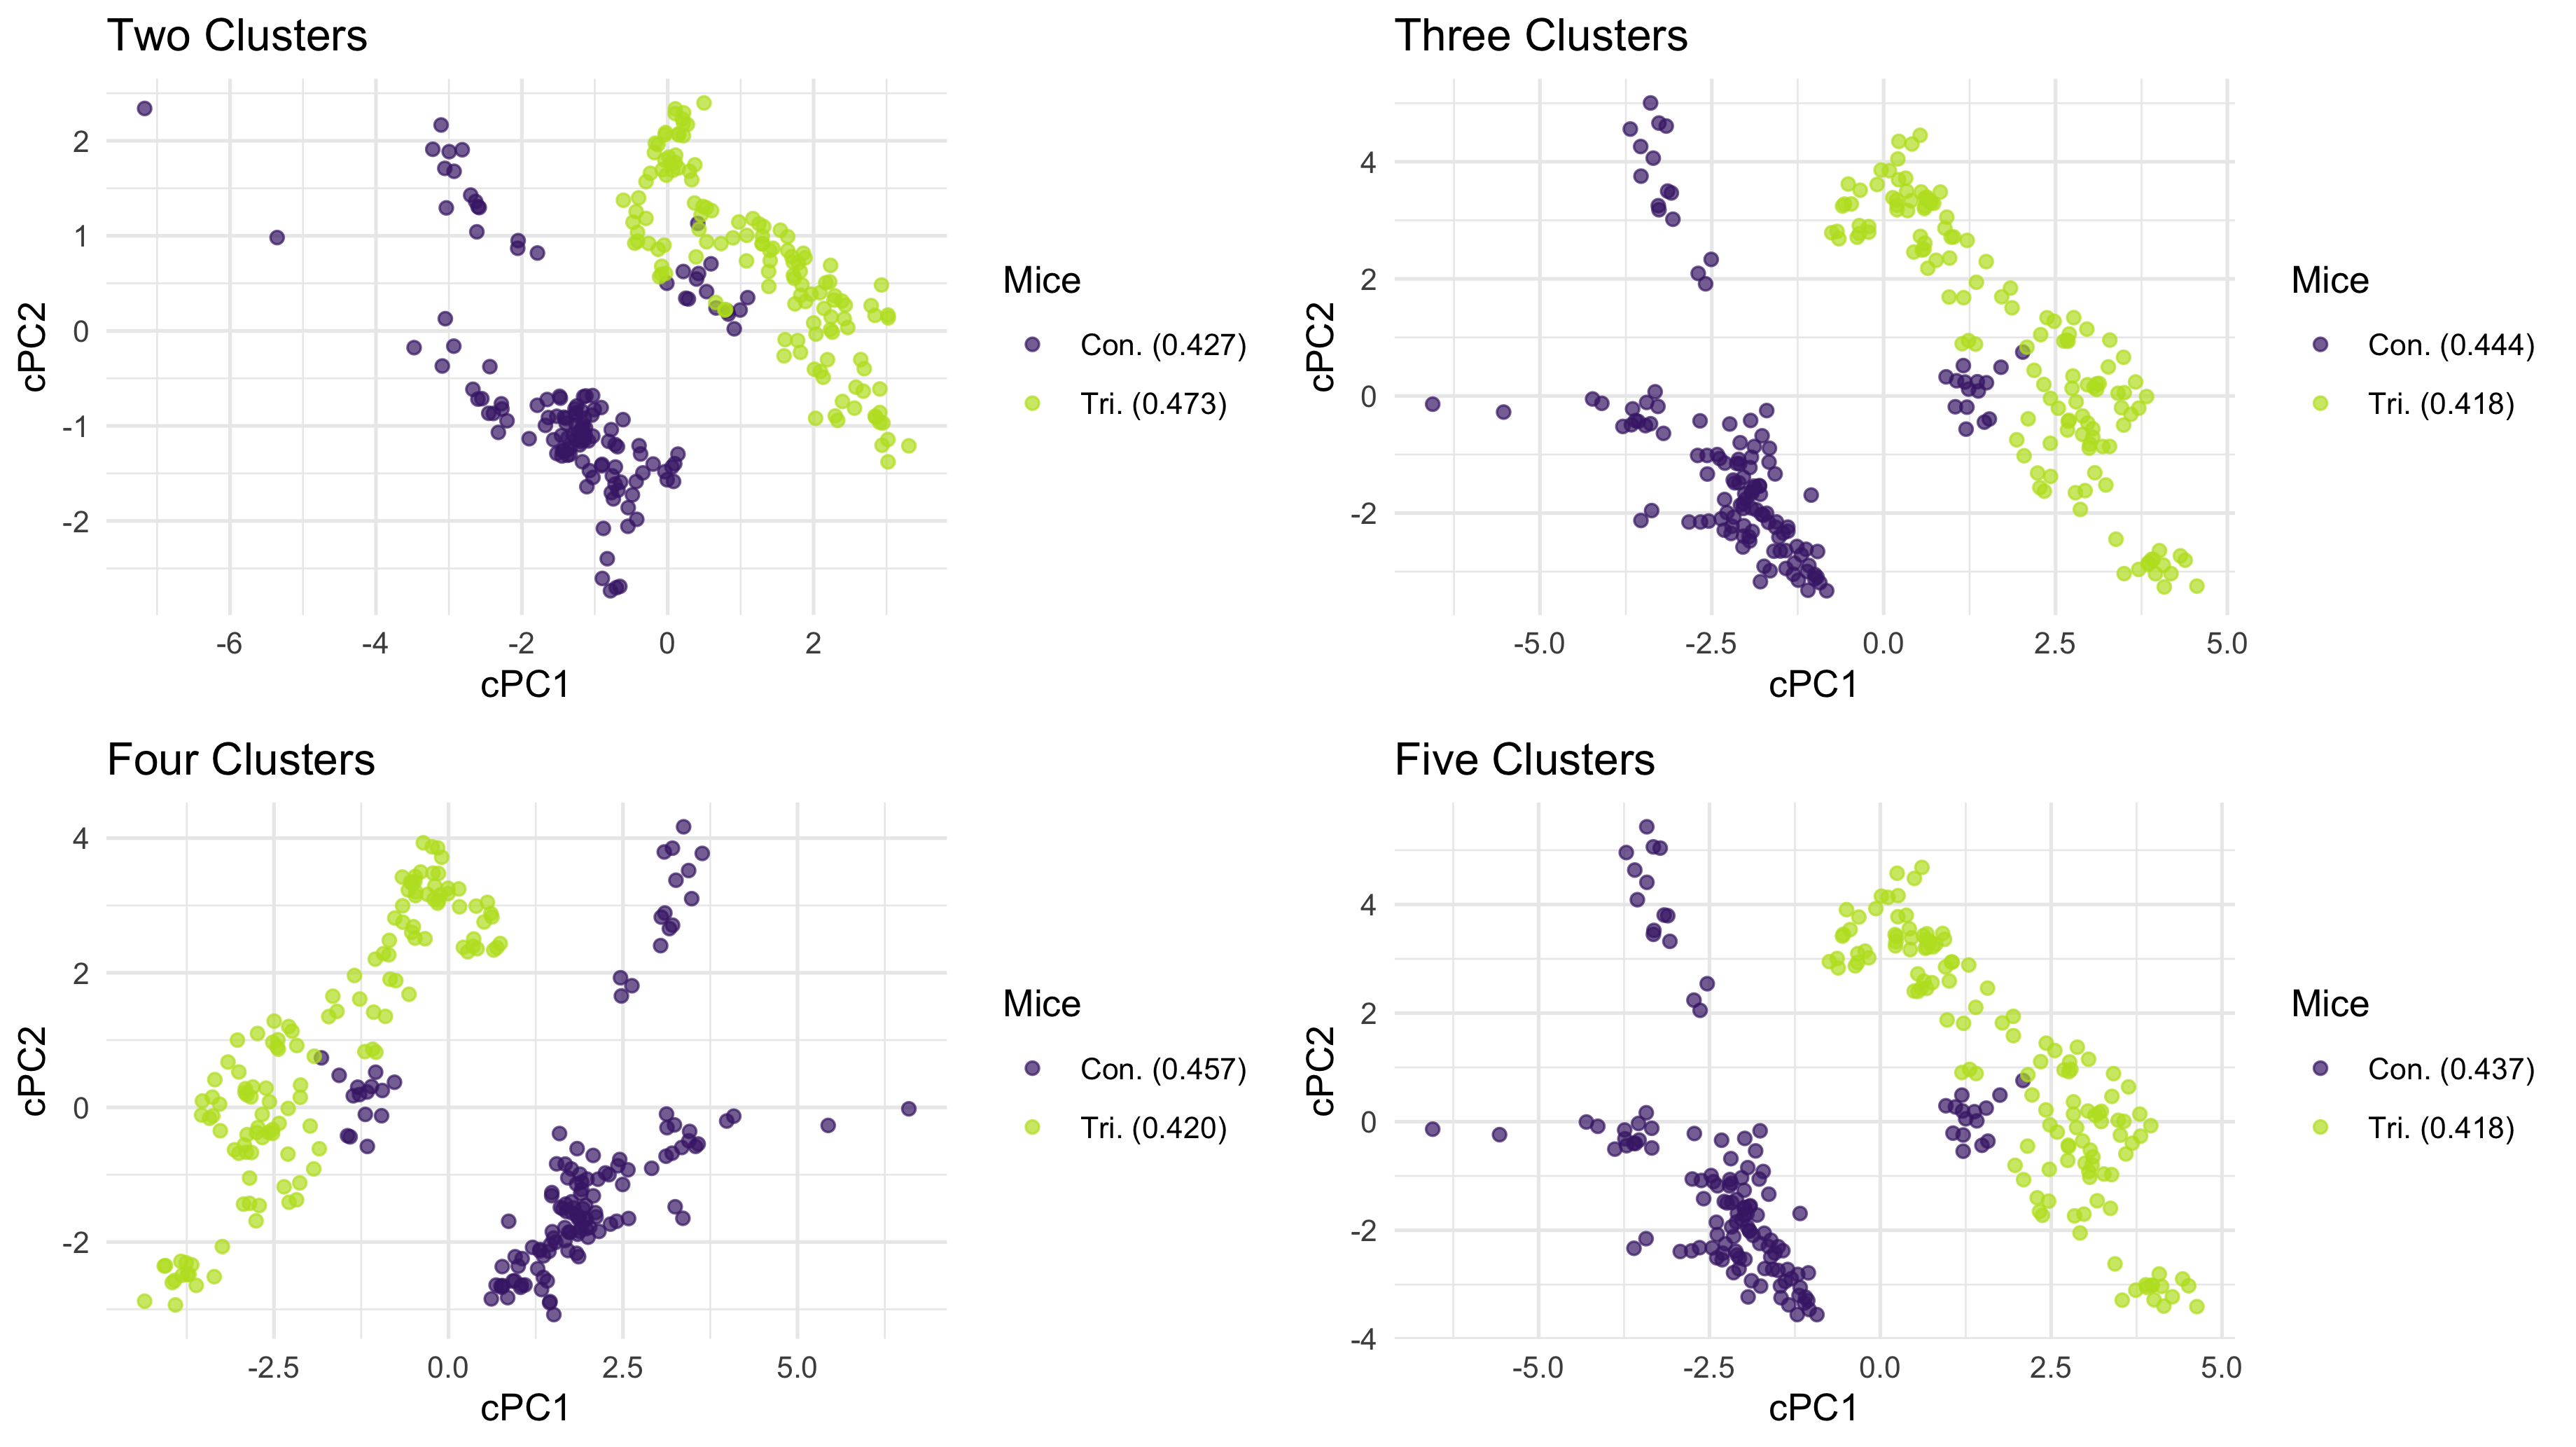
\includegraphics[width=0.9\textwidth]{figures/mice_cpca_centers}
    \caption{
    \textit{Mouse protein expression data: cPCA.}
    When varying the \textit{a priori} specified number of clusters for cPCA, we find that the two-dimensional embedding is once again robust to misspecifications.
    }
    \label{fig:mice_cpca_centers}
\end{figure}

\begin{figure}[!htbp]
    \centering
    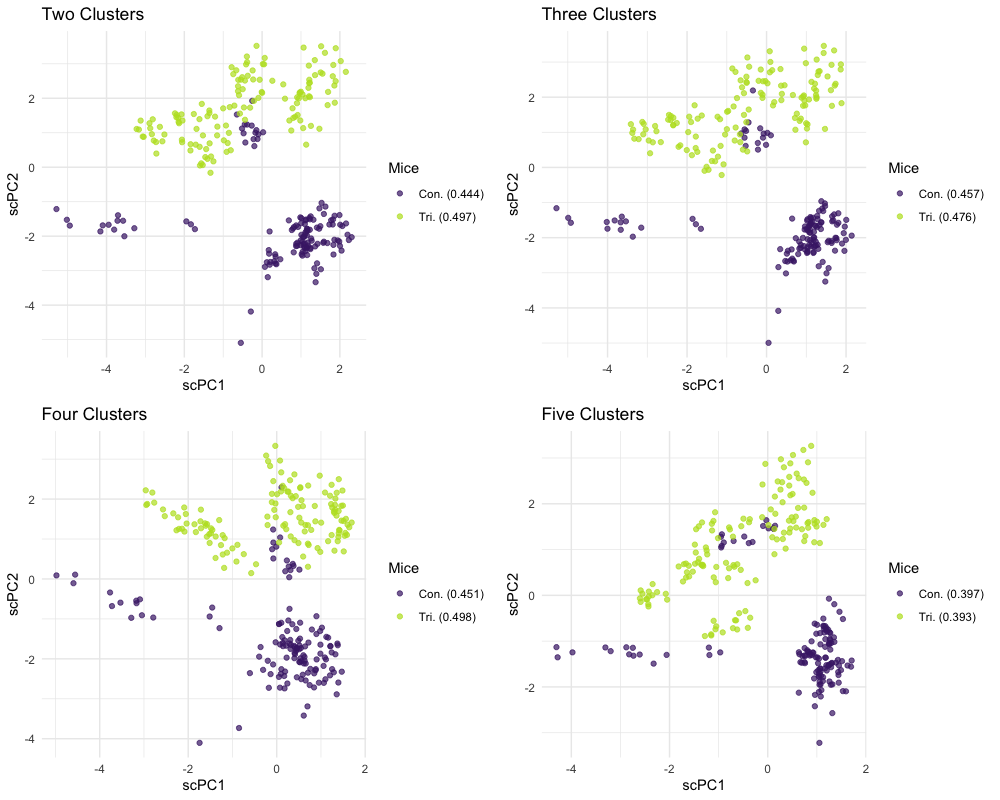
\includegraphics[width=0.9\textwidth]{figures/mice_scpca_centers}
    \caption{
    \textit{Mouse protein expression data: scPCA.}
    Unlike with the dengue microarray data, when varying the \textit{a priori} specified number of clusters for scPCA, we find that the two-dimensional embedding is robust to misspecifications. This may indicate that the sensitivity of the method to this tuning parameter is data-dependent.
    }
    \label{fig:mice_scpca_centers}
\end{figure}

\begin{longtable}{| l | p{4cm} | l |}
  \caption{{\em Mouse protein expression data: Proteins with non-zero weights in the first scPCA loadings vector.}} \label{tab:mouse_prot_1} \\
  \hline
   & Protein Symbol & Weight \\ 
 \hline
  1 & ELK & 0.0618 \\ 
  2 & BRAF & -0.1001 \\ 
  3 & RSK & -0.0927 \\ 
  4 & SOD1 & 0.1800 \\ 
  5 & S6 & 0.1281 \\ 
  6 & AcetylH3K9 & 0.3992 \\ 
  7 & RRP1 & 0.0606 \\ 
  8 & Tau & 0.7320 \\ 
  9 & CASP9 & -0.0795 \\ 
  10 & PSD95 & -0.0329 \\ 
  11 & Ubiquitin & -0.3674 \\ 
  12 & H3AcK18 & 0.2958 \\ 
 \hline
 \end{longtable}

\newpage
\begin{longtable}{| l | p{4cm} | l |}
  \caption{{\em Mouse protien expression data: Proteins with non-zero weights in the second scPCA loadings vector.}}
  \label{tab:mouse_prot_2} \\
  \hline
 & Protein Symbol & Weight \\ 
 \hline
  1 & ELK & -0.2236 \\ 
  2 & AKT & -0.0999 \\ 
  3 & APP & 0.3525 \\ 
  4 & SOD1 & -0.2323 \\ 
  5 & NUMB & 0.4690 \\ 
  6 & P70S6 & 0.1554 \\ 
  7 & GSK3B & 0.3574 \\ 
  8 & PKCG & 0.3978 \\ 
  9 & S6 & 0.3674 \\ 
  10 & RRP1 & 0.0272 \\ 
  11 & GluR4 & 0.0404 \\ 
  12 & IL1B & -0.2664 \\ 
  13 & P3525 & 0.0196 \\ 
  14 & PSD95 & -0.1289 \\ 
  15 & SNCA & -0.0783 \\ 
  16 & H3AcK18 & 0.0169 \\ 
 \hline
 \end{longtable}
 
\newpage
\bibliographystyleSM{natbib}
\bibliographySM{references}

 \end{document}